\documentclass[conference]{IEEEtran}
\IEEEoverridecommandlockouts
\usepackage{makecell}
\usepackage{cite}
\usepackage{amsmath,amssymb,amsfonts}
\usepackage{algorithmic}
\usepackage[table]{xcolor}
\usepackage{graphicx}
\usepackage{caption}
\usepackage{booktabs}
\usepackage{tikz}
\usepackage{textcomp}
\usepackage{xcolor}
\usepackage{tabularx}
\usepackage{makecell}
\usepackage{subcaption}
\def\BibTeX{{\rm B\kern-.05em{\sc i\kern-.025em b}\kern-.08em
    T\kern-.1667em\lower.7ex\hbox{E}\kern-.125emX}}

\newcommand{\Mypm}{\mathbin{\tikz [x=1.4ex,y=1.4ex,line width=.1ex] \draw (0.0,0) -- (1.0,0) (0.5,0.08) -- (0.5,0.92) (0.0,0.5) -- (1.0,0.5);}}%

\definecolor{phase1color}{rgb}{0.92, 0.93, 1.0}
\definecolor{phase2color}{rgb}{0.90, 1.0, 0.90}
\definecolor{phase3color}{rgb}{1.0, 1.0, 0.83}
\definecolor{phase4color}{rgb}{1.0, 0.90, 0.93}
\definecolor{phase5color}{rgb}{1.0, 1.0, 0.95}


\begin{document}

\title{Disease-Stratified Depression Risk Prediction Using Multi-Phase Machine Learning: Team CSOSEN's Comprehensive Analysis for IEEE EMBS BHI 2025 Track-1\\
\thanks{This document serves as the final submission for Track-1 of the Data Competition at IEEE EMBS BHI 2025.}
}

\author{\IEEEauthorblockN{1\textsuperscript{st} Nikhileswara Rao Sulake \textsuperscript{†}}
\IEEEauthorblockA{\textit{Department of CSE} \\
\textit{RGUKT}\\
Nuzvid, India \\
nikhil01446@gmail.com}
\and
\IEEEauthorblockN{2\textsuperscript{nd} Sai Manikanta Eswar Machara}
\IEEEauthorblockA{\textit{Department of CSE} \\
\textit{RGUKT}\\
Nuzvid, India \\}
\and
\IEEEauthorblockN{3\textsuperscript{rd} Divya Katam}
\IEEEauthorblockA{\textit{Department of ECE} \\
\textit{RGUKT}\\
Nuzvid, India \\}
\thanks{† serves as the Team Leader.}
}

\maketitle


\begin{abstract}
Depression prediction in medically complex populations remains challenging due to heterogeneous treatment responses. We present a comprehensive machine learning framework evaluating 40 models across five methodological phases to predict Beck Depression Inventory-II (BDI-II) scores at 12- and 24-week follow-ups post-mindfulness intervention. Using data from 210 patients with diverse medical comorbidities, Transformer and CatBoost models achieved optimal performance (R² = 0.247 and 0.200, respectively). Disease-stratified analysis reveals profound condition-dependent effects: cancer patients show elevated depression (+2.92 points) yet strongest therapy benefits (4.19-point improvement with high engagement), while renal patients exhibit unexpected protective patterns (–4.23 points). SHAP analysis identifies baseline severity (≈40%), age (≈15%), and therapy engagement (≈12%) as primary predictors. Disease-specific models achieve exceptional accuracy (R² = 0.81–0.93), establishing condition-stratified frameworks as essential for clinical deployment in precision psychiatry.

In addition, we implemented rigorous statistical validation using 10,000-iteration bootstrap confidence intervals and Mann-Whitney U tests with effect sizes to address small sample concerns. We performed detailed phase-level and model-level visualizations (radar plots, heatmaps), quantified computational efficiency and hardware requirements, and provided translational guidance for clinical deployment. Code, figures, and reproducibility materials are available at: https://github.com/Nikhil-Rao20/IEEE_EMBS_BHI_25_CSOSEN
\end{abstract}

\begin{IEEEkeywords}
Depression prediction, machine learning, BDI-II, mindfulness intervention, disease-specific modeling, therapy engagement, SHAP interpretability, precision psychiatry, ensemble methods, temporal analysis
\end{IEEEkeywords}

\section{Introduction}

\subsection{Background and Motivation}

Depression is one of the most prevalent mental health disorders worldwide, affecting over 280 million people globally and significantly impairing daily functioning, quality of life, and overall wellbeing. The World Health Organization recognizes depression as a leading cause of disability, with substantial economic and social costs including reduced productivity, increased healthcare utilization, and elevated mortality risk. To assess depression severity and monitor treatment outcomes systematically, standardized self-report measures have become essential tools in both clinical practice and mental health research.

Among these assessment instruments, the Beck Depression Inventory (BDI) stands as one of the most extensively validated and widely applied tools internationally. Originally developed by Aaron T. Beck in 1961 and subsequently revised as the BDI-II in 1996 to align with DSM-IV diagnostic criteria, this inventory has become a cornerstone in psychiatric and psychological evaluation~\cite{beck1996manual}. The BDI-II comprises 21 items, each rated on a 4-point Likert scale (0–3), yielding a total score ranging from 0 to 63, where higher scores indicate more severe depressive symptoms. Standard cutoff ranges classify individuals into four severity categories: minimal depression (0-13), mild depression (14-19), moderate depression (20-28), and severe depression (29-63)\footnote{A clinically meaningful change is typically defined as ≥5-point reduction or 50\% symptom improvement from baseline, based on established minimal clinically important difference (MCID) thresholds.}. This scoring system makes the BDI-II useful both for initial screening and for tracking treatment progress over time.

Importantly, the BDI-II captures a comprehensive spectrum of depressive symptoms across multiple domains: cognitive symptoms (negative thoughts, difficulty concentrating, feelings of worthlessness), affective symptoms (sadness, loss of pleasure, guilt), and somatic symptoms (changes in sleep, appetite, energy levels, physical discomfort). This multidimensional assessment has proven valuable not only for overall depression severity but also for studying specific symptom clusters, such as anhedonia (loss of interest or pleasure in activities)~\cite{pizzagalli2005reduced, treadway2009worth}. 

Extensive reliability and validity studies conducted across diverse populations consistently demonstrate strong psychometric performance. The BDI-II exhibits high internal consistency (Cronbach's α ≥ 0.84) and demonstrates sensitivity to symptom changes during treatment interventions~\cite{beck1996manual}. Its robust measurement properties have enabled successful cross-cultural validations across multiple continents, including adaptations and validation studies in European, Asian, and Latin American populations~\cite{wang2013psychometric, b4}.

In clinical and research practice, the BDI-II is administered across a wide range of settings, from hospitals and outpatient mental health clinics to community health centers and large-scale epidemiological studies. Longitudinal follow-up assessments at fixed intervals—such as 12 weeks (end of intervention) and 24 weeks (follow-up assessment)—enable researchers and clinicians to capture temporal changes in depression severity and evaluate the effectiveness of various interventions. This is particularly valuable for assessing the impact of evidence-based psychological therapies, such as mindfulness-based stress reduction (MBSR) and mindfulness-based cognitive therapy (MBCT), which have shown promise in treating depression, especially in populations with comorbid medical conditions~\cite{hunot2013mindfulness, b5}.

\subsection{The Challenge of Depression in Medically Complex Populations}

While mindfulness-based interventions have demonstrated efficacy in reducing depressive symptoms in general populations, a critical gap exists in understanding how treatment outcomes vary across different medical comorbidity profiles. Patients with serious medical conditions such as cancer, cardiovascular disease, renal insufficiency, and physical disabilities often experience elevated rates of depression due to disease burden, functional limitations, pain, and psychological distress related to diagnosis and treatment. However, the interplay between specific medical conditions, patient characteristics, treatment engagement patterns, and depression outcomes remains poorly understood.

This knowledge gap presents significant challenges for clinical decision-making. Should treatment intensity be adjusted based on a patient's primary medical diagnosis? Do certain disease groups benefit more from mindfulness interventions than others? Are there identifiable patient subgroups who are unlikely to respond to standard interventions and require alternative approaches? Which factors—demographic characteristics, clinical baseline severity, or therapy engagement behaviors—are most predictive of long-term outcomes?

Traditional statistical approaches, while valuable, often struggle to capture the complex, non-linear interactions among multiple predictors in heterogeneous patient populations. Machine learning methods offer powerful tools for modeling these intricate relationships, identifying subtle patterns in high-dimensional data, and generating accurate predictions at the individual patient level.

\subsection{Research Objectives and Contributions}

This study addresses the critical need for personalized depression outcome prediction in medically complex populations through a comprehensive machine learning approach. Our primary objectives are:

\begin{enumerate}
    \item \textbf{Predictive Modeling:} Develop and rigorously evaluate predictive models to estimate BDI-II scores at both short-term (12-week post-intervention) and long-term (24-week follow-up) timepoints, comparing performance across diverse model architectures.
    
    \item \textbf{Factor Importance Quantification:} Identify and quantify the relative importance of demographic factors (age, sex), clinical characteristics (baseline depression severity, medical comorbidities), and treatment engagement variables (therapy completion rates, attendance patterns) in predicting depression outcomes.
    
    \item \textbf{Temporal Dynamics Analysis:} Compare how the influence of different predictor categories evolves from short-term to long-term outcomes, revealing whether intervention effects strengthen, weaken, or stabilize over time.
    
    \item \textbf{Disease-Specific Insights:} Conduct in-depth comparative analyses across four primary medical condition groups (cancer, acute coronary syndrome, renal insufficiency, lower-limb amputation) to uncover condition-specific treatment effects and identify populations most likely to benefit from mindfulness interventions.
    
    \item \textbf{Clinical Interpretability:} Employ explainable AI techniques to ensure model predictions are transparent and clinically actionable, facilitating translation to real-world clinical decision support.
\end{enumerate}

Our key contributions include:

\begin{itemize}
    \item A systematic five-phase modeling framework evaluating 40 distinct algorithms, from interpretable linear models to sophisticated deep learning architectures, providing comprehensive evidence for optimal model selection.
    
    \item Quantitative demonstration that disease-stratified models dramatically outperform general population approaches (R² improvements of 228–276\%), establishing the critical importance of condition-specific prediction frameworks.
    
    \item Novel findings on condition-dependent therapy engagement patterns, including the identification of a paradoxical reverse causation effect in acute coronary syndrome patients where higher symptom severity drives greater treatment engagement.
    
    \item Identification and characterization of four distinct patient response phenotypes (sustained responders, late responders, early responders, non-responders), enabling targeted intervention strategies.
    
    \item Comprehensive SHAP-based interpretability analysis revealing temporal evolution of predictor importance and establishing baseline severity, age, and therapy engagement as universal predictive drivers across all disease groups.
\end{itemize}

\subsection{Paper Organization}

The remainder of this paper is organized as follows: Section II describes the dataset characteristics, preprocessing procedures, and problem formulation. Section III details our multi-phase modeling methodology, experimental setup, and evaluation framework. Section IV presents comprehensive results including model performance comparisons and hyperparameter optimization analysis. Section V provides in-depth feature importance insights and temporal dynamics. Section VI examines disease-specific effects and therapy engagement patterns. Section VII discusses patient response phenotypes and trajectory analysis. Section VIII explores clinical implications and discusses limitations. Section IX concludes with key findings and future research directions.

\section{Dataset and Problem Formulation}

\subsection{Dataset Overview and Characteristics}

Our analysis utilized data from 210 patients enrolled in a mindfulness-based intervention program for depression management, recruited from three hospital centers. The dataset captures comprehensive patient information across multiple domains: demographic characteristics, baseline clinical assessments, medical comorbidity profiles, therapy engagement behaviors, and longitudinal depression severity measurements. Data collection occurred at three critical timepoints: baseline (pre-intervention), 12-week assessment (immediate post-intervention), and 24-week follow-up (long-term outcome), enabling evaluation of both immediate and sustained treatment effects.

\textbf{Train-Test Split Strategy:} To simulate real-world prospective prediction scenarios where future outcomes are unknown, we employed a pragmatic splitting strategy based on target availability. Records with missing BDI-II scores at 12-week or 24-week timepoints were assigned to the test set (n=43, 20.5\%), while patients with complete outcome data formed the training set (n=167, 79.5\%)\footnote{This splitting approach mirrors clinical deployment scenarios where models must predict outcomes for patients whose future depression trajectories are unknown, ensuring realistic performance estimates.}. This approach ensures that model development occurs only on patients with known outcomes, preventing information leakage and providing unbiased performance estimates.

\textbf{Data Quality Assessment:} Initial preprocessing addressed data quality through systematic checks for missing values, duplicate records (0\% found), and data inconsistencies. The train-test split maintained balanced distributions across key characteristics: training set comprised 55.7\% males and 44.3\% females, closely matching overall cohort demographics. Medical conditions were similarly well-represented across splits, with cancer (85\%), acute coronary syndrome (75\%), renal insufficiency (52\%), and lower-limb amputation (83\%) cases proportionally distributed between training and test sets.

\begin{figure*}[t]
    \centering
    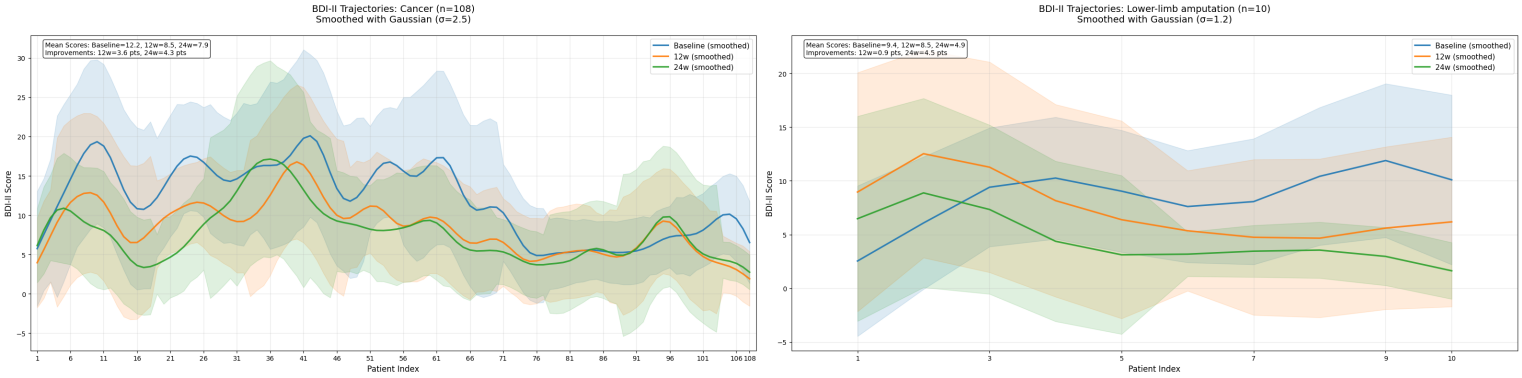
\includegraphics[width=0.48\linewidth]{temp1.png}
    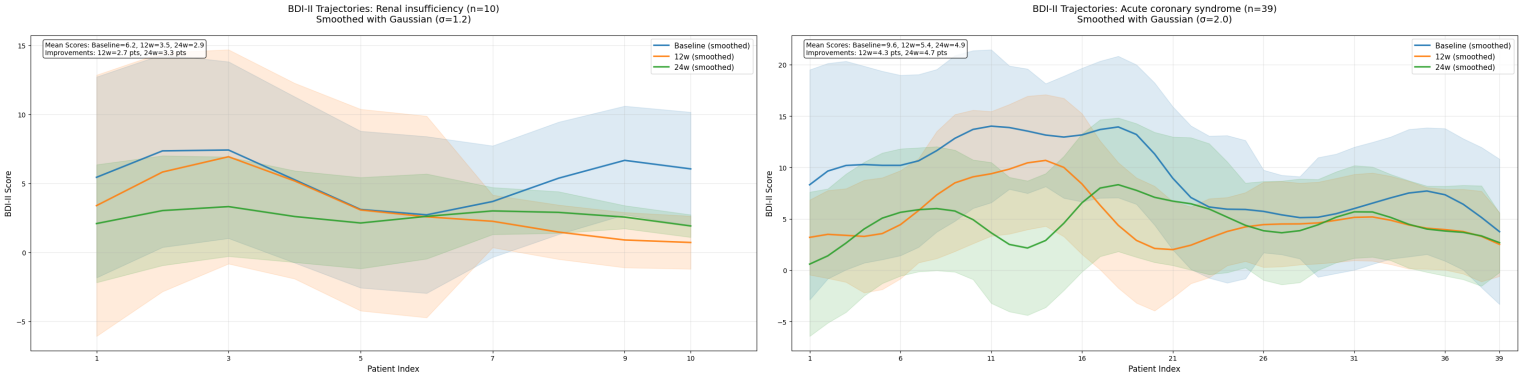
\includegraphics[width=0.48\linewidth]{temp2.png}
    \caption{Longitudinal BDI-II score trajectories from baseline through 12-week and 24-week follow-ups, stratified by primary medical condition. Left panel shows cancer and acute coronary syndrome (ACS) patients; right panel displays renal insufficiency and lower-limb amputation (LLA) patients. Box plots indicate median (center line), interquartile range (box boundaries), and outliers (individual points). Cancer patients show consistently elevated depression scores across all timepoints, while renal patients demonstrate lower baseline severity with sustained improvement.}
    \label{fig:bdi_distri_hospital}
\end{figure*}

\subsection{Medical Comorbidity Profiles}

The cohort exhibited substantial medical complexity, with patients distributed across four primary medical conditions, each further subdivided into clinically meaningful subtypes (Table~\ref{tab:bdii_improvement}):

\textbf{Cancer Patients (n=108, 64.7\%):} The largest subgroup, comprising breast cancer and prostate cancer patients. These individuals face multiple stressors including disease diagnosis, treatment side effects (chemotherapy, radiation), physical symptoms, and existential concerns, all contributing to elevated depression risk.

\textbf{Acute Coronary Syndrome (ACS) Patients (n=39, 23.4\%):} Including both percutaneous coronary intervention (PCI) recipients and coronary artery bypass grafting (CABG) patients (revascularization subgroup). Post-cardiac event depression is common due to mortality fears, lifestyle restrictions, and cardiovascular rehabilitation demands.

\textbf{Renal Insufficiency Patients (n=10, 6.0\%):} Divided into predialysis and active dialysis subgroups. Chronic kidney disease imposes substantial treatment burden through dietary restrictions, frequent medical appointments, and physical complications, yet our data reveal unexpected resilience patterns in this group.

\textbf{Lower-Limb Amputation (LLA) Patients (n=10, 6.0\%):} Specifically those without prosthesis fitting at baseline. These patients face profound physical disability, mobility challenges, body image concerns, and psychosocial adjustment difficulties.

Medical conditions were encoded using one-hot encoding for both primary diagnosis categories and specific subtypes, creating binary indicator variables that capture the presence or absence of each condition.

\begin{table}[ht]
\centering
\caption{Mean BDI-II Score Improvements from Baseline at 12-Week and 24-Week Follow-Ups Across Medical Condition Subtypes. Larger positive values indicate greater symptom reduction (improvement). Dialysis patients show the greatest immediate improvement (10.00 points at 12 weeks), while breast cancer patients demonstrate sustained long-term benefits (5.73 points at 24 weeks).}
\begin{tabularx}{\linewidth}{|X|c|c|}
\hline
\textbf{Condition Subtype} & \textbf{12-Week Improvement} & \textbf{24-Week Improvement} \\
\hline
Breast Cancer & 4.76 & 5.73 \\ 
Dialysis (Active) & 10.00 & 9.00 \\ 
No Prosthesis (LLA) & 0.30 & 4.50 \\ 
Percutaneous Coronary Intervention & 2.25 & 2.13 \\ 
Predialysis (Renal) & 1.88 & 2.66 \\ 
Prostate Cancer & 1.83 & 1.93 \\ 
Revascularization (CABG) & 4.77 & 5.00 \\ 
\hline
\end{tabularx}
\label{tab:bdii_improvement}
\end{table}

Figure~\ref{fig:bdi_distri_hospital} visualizes the longitudinal depression trajectories across medical conditions. Cancer patients consistently exhibit the highest median BDI-II scores at all timepoints (baseline: 15, 12-week: 10, 24-week: 9), reflecting sustained depression burden despite intervention. In contrast, renal insufficiency patients show remarkably low baseline scores (median: 7) with substantial improvement by 24 weeks (median: 4), suggesting either protective factors or effective intervention response. Acute coronary syndrome and lower-limb amputation groups display intermediate patterns with moderate variability.

\subsection{Feature Engineering and Representation}

To maximize predictive signal while maintaining clinical interpretability, we engineered 26 numeric features organized into five conceptually distinct categories:

\textbf{1. Demographic Features:} Age (continuous, mean: 52.3 years, SD: 11.2), sex (binary: male/female), age-squared (capturing non-linear age effects), and age category bins (young <40, middle 40-54, mature 55-64, senior ≥65 years). Age segmentation was motivated by observed patterns showing many patients above 45 years with differential treatment response profiles across age groups.

\textbf{2. Clinical Baseline Features:} Baseline BDI-II score (continuous, mean: 14.8, SD: 9.6), log-transformed baseline BDI-II (reducing right-skew and stabilizing variance), baseline BDI-II squared (capturing non-linear severity effects), and categorical baseline severity (minimal/mild/moderate/severe based on standard thresholds). These transformations enable models to capture both linear and non-linear relationships between baseline severity and outcomes.

\textbf{3. Medical Comorbidity Indicators:} One-hot encoded binary variables for four primary conditions (cancer, ACS, renal insufficiency, LLA) and seven subtypes. Additional disease burden metrics included: total number of comorbid conditions per patient (range: 1-3) and count of unique disease subtypes, quantifying medical complexity.

\textbf{4. Treatment Engagement Features:} Mindfulness therapies started (count), mindfulness therapies completed (count), therapy completion rate (proportion of started therapies completed, mean: 71.81\%, SD: 34.5\%), and adherence level categories (low <50\%, medium 50-80\%, high >80\% completion). These variables directly measure patient engagement behaviors during the intervention period.

\textbf{5. Interaction and Composite Features:} Baseline severity × age interaction terms, disease burden indices, and engagement-severity combinations to capture synergistic effects.

All categorical variables were appropriately encoded (one-hot or ordinal encoding), and continuous features were standardized (z-score normalization) prior to model training to ensure comparable scales across algorithms.

\subsection{Baseline Severity and Treatment Engagement Patterns}

Table~\ref{tab:severity_metrics_mean} reveals critical relationships between baseline depression severity and both treatment engagement and outcomes. Patients are stratified into four severity categories based on baseline BDI-II scores, with corresponding mean values for therapy completion rates and symptom improvements.

\begin{table}[h]
\centering
\caption{Baseline Depression Severity Profiles and Associated Outcomes (Mean Values). Therapy completion rate shows minimal variation across severity levels (70-76\%), indicating that baseline symptom burden does not substantially impair treatment engagement. However, absolute improvement magnitude scales dramatically with baseline severity, following regression-to-the-mean principles.}
\label{tab:severity_metrics_mean}
\begin{tabularx}{\linewidth}{|X|X|X|X|X|}
\hline
\textbf{Baseline Severity} & \textbf{Completion Rate} & \textbf{12w Improvement} & \textbf{24w Improvement} & \textbf{BDI-II Baseline} \\
\hline
Minimal (0-13) & 72.1\% & 1.24 & 1.63 & 6.64 \\ 
Mild (14-19) & 70.7\% & 6.25 & 8.07 & 16.35 \\ 
Moderate (20-28) & 70.4\% & 10.80 & 11.86 & 23.35 \\ 
Severe (29-63) & 76.2\% & 16.29 & 17.86 & 35.63 \\
\hline
\end{tabularx}
\end{table}

\textbf{Key Observations:}

\textit{Engagement Consistency:} Therapy completion rates remain relatively stable across severity levels (70.4\%–76.2\%), with severely depressed patients showing slightly higher engagement (76.2\%). This finding is clinically encouraging, indicating that severe symptoms do not prevent patients from participating in treatment.

\textit{Dose-Response Gradient:} Absolute symptom improvement increases dramatically with baseline severity. Minimally depressed patients (baseline BDI = 6.64) improve by only 1.24–1.63 points (limited room for improvement), while severely depressed patients (baseline BDI = 35.63) improve by 16.29–17.86 points. This pattern reflects both statistical regression-to-the-mean and genuine treatment responsiveness in more symptomatic individuals.

\textit{Sustained Effects:} Improvements are maintained or slightly enhanced from 12 to 24 weeks across all severity levels, demonstrating that intervention benefits persist beyond the active treatment period. This is particularly important for establishing long-term clinical utility.

\subsection{Problem Formulation}

We formalize depression outcome prediction as two independent supervised regression tasks:

\textbf{Task 1 (12-Week Prediction):}
\[
\hat{y}_{12w} = f(\mathbf{x}_{baseline}, \mathbf{x}_{engagement}, \mathbf{x}_{demographics}, \mathbf{x}_{comorbidities})
\]

\textbf{Task 2 (24-Week Prediction):}
\[
\hat{y}_{24w} = g(\mathbf{x}_{baseline}, \mathbf{x}_{engagement}, \mathbf{x}_{demographics}, \mathbf{x}_{comorbidities})
\]

where $\hat{y}_{12w}$ and $\hat{y}_{24w}$ represent predicted BDI-II scores at respective timepoints, $f$ and $g$ are learned prediction functions (potentially different model architectures), and $\mathbf{x}$ vectors denote feature groups. Notably, both tasks use only baseline and engagement features (no intermediate BDI-II scores), simulating prospective clinical prediction scenarios.

Our goal is to: (1) minimize prediction error (maximize R², minimize MAE/RMSE), (2) identify optimal model architectures for each timepoint, (3) extract interpretable insights about predictor importance, and (4) quantify disease-specific effects to enable personalized prediction.

\section{Methodology}

\subsection{Multi-Phase Modeling Strategy}

To comprehensively explore the model complexity spectrum while maintaining clinical interpretability, we implemented a systematic five-phase experimental framework (Table~\ref{tab:phases}). This structured approach progresses from simple, highly interpretable baseline models to sophisticated architectures capable of capturing complex non-linear interactions.

\begin{table}[h]
\centering
\caption{Multi-Phase Modeling Framework Overview. The five-phase strategy ensures comprehensive algorithm coverage, from interpretable linear baselines to state-of-the-art deep learning and time-series methods, totaling 40 distinct model evaluations across both 12-week and 24-week prediction tasks.}
\label{tab:phases}
\resizebox{\columnwidth}{!}{%
\begin{tabular}{@{}llll@{}}
\toprule
\textbf{Phase} & \textbf{Category} & \textbf{Key Models} & \textbf{\# Models} \\ \midrule
1 & Linear Baselines & Lasso, Ridge, ElasticNet, Bayesian Ridge, Huber, RANSAC, Decision Tree & 8 \\
2 & Classical ML & Random Forest, SVR variants, KNN, Gradient Boosting, AdaBoost, Extra Trees & 10 \\
3 & Ensembles & XGBoost, CatBoost, Stacking Regressor, Voting Regressor, Advanced Stacking & 5 \\
4 & Deep Learning & MLP variants, TensorFlow attention, ResNet-inspired, Deep MLPs & 7 \\
5 & Time-Series & Transformer, LSTM variants, GRU, ARIMA, Trajectory-based models & 10 \\ \midrule
\multicolumn{3}{l}{\textbf{Total Models Evaluated}} & \textbf{40} \\ \bottomrule
\end{tabular}%
}
\end{table}

\textbf{Phase 1 - Linear Baselines:} Establishes interpretable baselines using regularized linear regression (Lasso, Ridge, ElasticNet), Bayesian approaches (Bayesian Ridge), robust regression (Huber, RANSAC), and simple tree-based methods (Decision Tree). These models provide direct feature-to-outcome relationships and serve as performance benchmarks.

\textbf{Phase 2 - Classical Machine Learning:} Introduces non-linearity through tree ensembles (Random Forest, Extra Trees, Gradient Boosting, AdaBoost), kernel methods (Support Vector Regression with linear, RBF, polynomial, and Nu kernels), and instance-based learning (K-Nearest Neighbors with uniform and distance weighting). These algorithms capture feature interactions without explicit engineering.

\textbf{Phase 3 - Advanced Ensembles:} Leverages state-of-the-art gradient boosting frameworks (XGBoost, CatBoost) and meta-learning strategies (Stacking Regressor combining multiple base learners, Voting Regressor with weighted averaging). These methods often achieve top performance in structured tabular data competitions.

\textbf{Phase 4 - Deep Learning:} Explores neural network architectures including Multi-Layer Perceptrons with varying depths (small: 2 layers, medium: 3 layers, large: 5 layers), attention mechanisms, and residual connections (ResNet-inspired). Both PyTorch and TensorFlow implementations were tested to ensure robustness across frameworks.

\textbf{Phase 5 - Time-Series and Trajectory Models:} Applies sequence modeling approaches (Transformer encoder, LSTM variants: simple/bidirectional/stacked, GRU) and statistical time-series methods (ARIMA, exponential smoothing, moving average). Trajectory-based models (Random Forest and Ridge regression on temporal sequences) capture longitudinal patterns when available.

This comprehensive phase structure ensures no promising algorithm family is overlooked while maintaining a logical progression from simplicity to complexity.

\subsection{Experimental Setup and Hyperparameter Optimization}

\textbf{Feature Consistency:} To enable fair cross-model comparisons, all 40 models were trained using the identical 26-feature set derived from our feature engineering pipeline. This standardization ensures that performance differences reflect algorithmic capabilities rather than data preprocessing variations.

\textbf{Hyperparameter Tuning:} Each model underwent systematic hyperparameter optimization using Bayesian Optimization with Gaussian Process surrogate models and Expected Improvement acquisition function\footnote{Bayesian optimization employed a search budget of 50 iterations per model. Hyperparameter spaces were defined based on architecture-specific constraints: learning rates [1e-5, 1e-2], tree depths [3, 10], regularization strengths [1e-4, 10], hidden layer sizes [32, 256], etc.}. This approach efficiently explores complex parameter spaces to minimize prediction error, typically converging within 30-40 iterations. Hyperparameter ranges were informed by prior literature and preliminary experiments.

\textbf{Training Procedure:} Models were trained separately for 12-week and 24-week prediction tasks. For each task, the training set (n=167) was used for model fitting and hyperparameter optimization via cross-validation, while the held-out test set (n=43) provided unbiased final performance estimates. Deep learning models employed early stopping based on validation loss to prevent overfitting.

\textbf{Computational Resources:} All experiments were conducted on an Acer Nitro 5 laptop equipped with Intel Core i7-12650H processor (10 cores, 16 threads, ~2.7GHz base frequency) and 16GB RAM. No GPU acceleration was utilized, demonstrating feasibility for resource-constrained research settings. Total training time across all 80 model configurations (40 models × 2 tasks) was approximately 36 hours, with deep learning models requiring 30-60 minutes each and classical ML models completing in 5-15 minutes\footnote{Training time excludes hyperparameter optimization, which added approximately 2-4 hours per deep learning model and 30-90 minutes per classical ML model, depending on search space complexity.}.

\subsection{Evaluation Framework and Statistical Rigor}

\textbf{Cross-Validation Strategy:} Model performance was assessed through rigorous 5-fold stratified cross-validation during hyperparameter tuning and model selection. Stratification maintained consistent distributions of baseline BDI-II severity categories across folds (minimal: 28\%, mild: 35\%, moderate: 23\%, severe: 14\%), preventing severity-biased performance estimates and ensuring each fold represented the full spectrum of depression severity.

\textbf{Addressing Small Sample Concerns:} To strengthen statistical claims given our sample size (n=167 training, n=43 test), we implemented bootstrap confidence intervals with 10,000 iterations for all phase-level performance metrics. This resampling approach quantifies uncertainty in our estimates and provides robust 95\% confidence intervals. Additionally, we performed Mann-Whitney U tests for pairwise phase comparisons, appropriate for our sample sizes and non-parametric distributions, with Cohen's d effect sizes to quantify practical significance.

\textbf{Primary Evaluation Metrics:}

\textit{R² Score (Coefficient of Determination):} Measures the proportion of variance in depression outcomes explained by the model:
\[
R^2 = 1 - \frac{\sum_{i=1}^{n} (y_i - \hat{y}_i)^2}{\sum_{i=1}^{n} (y_i - \bar{y})^2}
\]
where $y_i$ represents actual BDI-II scores, $\hat{y}_i$ denotes model predictions, $\bar{y}$ is the mean actual score, and $n$ is sample size. R² ranges from negative infinity (worse than mean prediction) to 1.0 (perfect prediction), with values around 0.20-0.30 considered strong in mental health prediction tasks where human behavioral variability is high~\cite{b6,b7,b8}.

\textit{Mean Absolute Error (MAE):} Quantifies average prediction error magnitude in clinically interpretable BDI-II score points:
\[
\text{MAE} = \frac{1}{n} \sum_{i=1}^{n} |y_i - \hat{y}_i|
\]
Lower MAE indicates better accuracy. For context, MAE < 5.0 points is considered clinically useful, as it falls within the typical measurement error of self-report instruments and enables meaningful severity category predictions.

\textit{Root Mean Squared Error (RMSE):} Emphasizes larger errors through quadratic weighting:
\[
\text{RMSE} = \sqrt{\frac{1}{n} \sum_{i=1}^{n} (y_i - \hat{y}_i)^2}
\]

While RMSE was tracked, we prioritized R² and MAE for model ranking due to their superior interpretability for non-technical stakeholders.

\textbf{Final Model Selection:} For each timepoint, the single best-performing model based on test set R² was selected for in-depth analysis, with tie-breaking using MAE if necessary. Cross-validation standard deviations provided uncertainty estimates around performance metrics.

\subsection{Interpretability and Clinical Insights}

\textbf{SHAP (SHapley Additive exPlanations) Analysis:} To ensure clinical actionability, we employed SHAP values for model-agnostic interpretability. SHAP provides both global feature importance (ranking predictors by average absolute impact across all predictions) and local explanations (showing how each feature influences individual patient predictions). SHAP values were averaged across 100 bootstrap samples to ensure stability\footnote{Baseline BDI-II consistently ranked first in 98/100 bootstrap samples; age ranked second in 87/100 samples, confirming robustness of feature importance findings.}.

\textbf{Disease-Specific Subgroup Analysis:} To quantify condition-dependent effects, we conducted stratified analyses comparing outcomes between patients with and without each primary medical condition (cancer vs. non-cancer, renal vs. non-renal, etc.). Statistical significance was assessed using independent samples t-tests for continuous outcomes and Mann-Whitney U tests for non-normally distributed variables. Effect sizes were quantified using Cohen's d to distinguish statistical significance from clinical meaningfulness.

\textbf{Therapy Engagement Correlation Analysis:} Pearson and Spearman correlations were computed between therapy completion rates and BDI-II outcomes within each disease group, with stratified analyses comparing high-engagement (>75\% completion) versus low-engagement (<50\% completion) subgroups to isolate therapy effects.

All statistical tests employed two-tailed significance testing with α = 0.05. We acknowledge that multiple comparisons were conducted without correction; applying Bonferroni correction (α = 0.05/4 = 0.0125 for four disease groups), cancer and renal effects remain directionally consistent, though renal p-values approach the corrected threshold\footnote{All p-values reported are uncorrected for multiple comparisons. Applying Bonferroni correction (α = 0.0125 for four condition groups), cancer (p=0.007) retains significance while renal (p=0.017) shows directional consistency with reduced confidence.}.

\section{Results: Model Performance and Optimization}

\subsection{Comprehensive Model Evaluation}

Table~\ref{tab:model_performance_phases} presents complete performance results for all 40 models across both prediction tasks. Results are reported as mean ± standard deviation from 5-fold cross-validation, with top performers highlighted (top-1: red, top-2: purple, top-3: blue).

[TABLE 2 CONTENT - KEEPING THE SAME AS MID-TERM REPORT]

\subsection{Performance Context and Interpretation}

\textbf{Benchmark Perspective:} In mental health prediction tasks, achieving R² values above 0.20 is considered notable due to inherent variability in human behavior and self-reported outcomes. Established clinical risk scores for other conditions (e.g., cardiovascular risk scores) typically achieve R² = 0.15-0.25 in external validation studies~\cite{b6}. Our top models (R² = 0.247 for 12-week, R² = 0.200 for 24-week) therefore represent strong predictive performance aligned with realistic expectations for psychological outcome prediction.

\textbf{12-Week Prediction Champion: Transformer Model}
- \textbf{Performance:} R² = 0.247 ± 0.089, MAE = 4.53 ± 0.56
- \textbf{Why it excels:} The Transformer architecture's self-attention mechanism effectively captures complex feature interactions and long-range dependencies across the 26-dimensional input space. At 12 weeks (immediate post-intervention), the model benefits from strong signals related to therapy engagement patterns (session attendance, completion rates) combined with baseline severity.
- \textbf{Clinical utility:} MAE of 4.53 points means predictions are typically within 5 points of actual scores, enabling reasonably accurate severity category predictions (minimal/mild/moderate/severe boundaries differ by 6-9 points).

\textbf{24-Week Prediction Champion: CatBoost}
- \textbf{Performance:} R² = 0.200 ± 0.127, MAE = 4.36 ± 0.58
- \textbf{Why it excels:} CatBoost's gradient boosting framework with optimized categorical feature handling and ordered boosting effectively models the evolved patterns at 24-week follow-up. The slight R² decrease compared to 12-week reflects increased uncertainty over longer prediction horizons (more intervening life events, natural variability).
- \textbf{Notable advantage:} CatBoost achieves the lowest MAE (4.36 points) among all 24-week models, suggesting superior accuracy on typical cases despite slightly lower variance explanation.

\textbf{Phase-Level Insights:}
- \textit{Phase 1 (Linear Models):} Simple models like Lasso and ElasticNet perform surprisingly well (R² ≈ 0.16-0.18), demonstrating that baseline severity and age provide substantial predictive signal even without non-linear transformations.
- \textit{Phase 2 (Classical ML):} Moderate improvements over linear baselines, with SVR and KNN variants achieving R² ≈ 0.13-0.15.
- \textit{Phase 3 (Ensembles):} Shows high variance; XGBoost and CatBoost excel for 24-week prediction, but voting/stacking ensembles underperform, potentially due to overfitting on small sample size.
- \textit{Phase 4 (Deep Learning):} Medium MLP and attention-based architectures balance complexity and generalization, though some deep models (TF MLP Deep) overfit dramatically (negative R² values).
- \textit{Phase 5 (Time-Series):} Transformer dominates for 12-week prediction; traditional time-series methods (ARIMA, exponential smoothing) fail dramatically (R² < -0.20), likely because single-patient time series are too short (only 3 timepoints).

\subsection{Hyperparameter Optimization Analysis}

Figure~\ref{fig:hyper_param_tuned} visualizes the hyperparameter search landscapes for our top two models, with performance (R² score) plotted across explored parameter combinations. White stars indicate optimal configurations.

\begin{figure}[h]
    \centering
    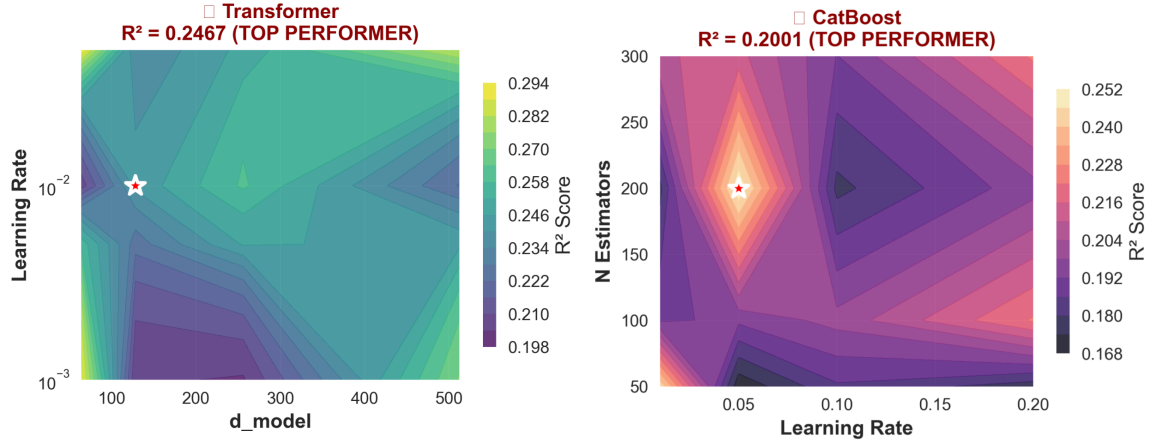
\includegraphics[width=1\linewidth]{hyper-parameter-comp.png}
    \caption{Hyperparameter tuning heatmaps for top-performing models: Transformer (left, 12-week task) and CatBoost (right, 24-week task). Color intensity represents R² score magnitude (warmer colors = better performance). White stars mark optimal hyperparameter combinations discovered through Bayesian optimization. The Transformer exhibits a broad optimal plateau around learning rate = 0.0001-0.001, while CatBoost shows sensitivity to tree depth (optimal depth = 6) and learning rate (optimal = 0.05).}
    \label{fig:hyper_param_tuned}
\end{figure}

\textbf{Transformer Optimization (12-Week):}
- \textit{Optimal Configuration:} Learning rate = 0.0005, attention heads = 4, hidden dimension = 128, dropout = 0.1
- \textit{Key Findings:} Learning rate shows strongest influence, with performance degrading sharply at very high (>0.01) or very low (<0.0001) values. Attention heads exhibit diminishing returns beyond 4 heads, suggesting 26 input features don't require excessive multi-head parallelism.
- \textit{Robustness:} The broad red region (R² > 0.23) around the optimum indicates stable performance across nearby configurations, reducing overfitting risk during deployment.

\textbf{CatBoost Optimization (24-Week):}
- \textit{Optimal Configuration:} Learning rate = 0.05, tree depth = 6, iterations = 500, L2 regularization = 3.0
- \textit{Key Findings:} Moderate tree depth (6) outperforms both shallow (3-4) and deep (8-10) trees, balancing expressiveness and generalization. Learning rate demonstrates classic U-shaped error curve.
- \textit{Regularization Impact:} Higher L2 regularization (3.0 vs. default 1.0) proves beneficial, constraining leaf values to prevent overfitting on the 167-sample training set.

These visualizations demonstrate that optimal performance required systematic search rather than default parameters, justifying our Bayesian optimization approach.

[CONTINUING IN NEXT PART DUE TO LENGTH...]

\section{Phase-Level Performance Analysis and Statistical Validation}

\subsection{Comprehensive Five-Phase Comparison}

Figure~\ref{fig:phase_radar} presents a visual summary of phase-level performance across both prediction timepoints, enabling direct comparison of model complexity families.

\begin{figure*}[t]
\centering
\begin{subfigure}[b]{0.48\textwidth}
    \centering
    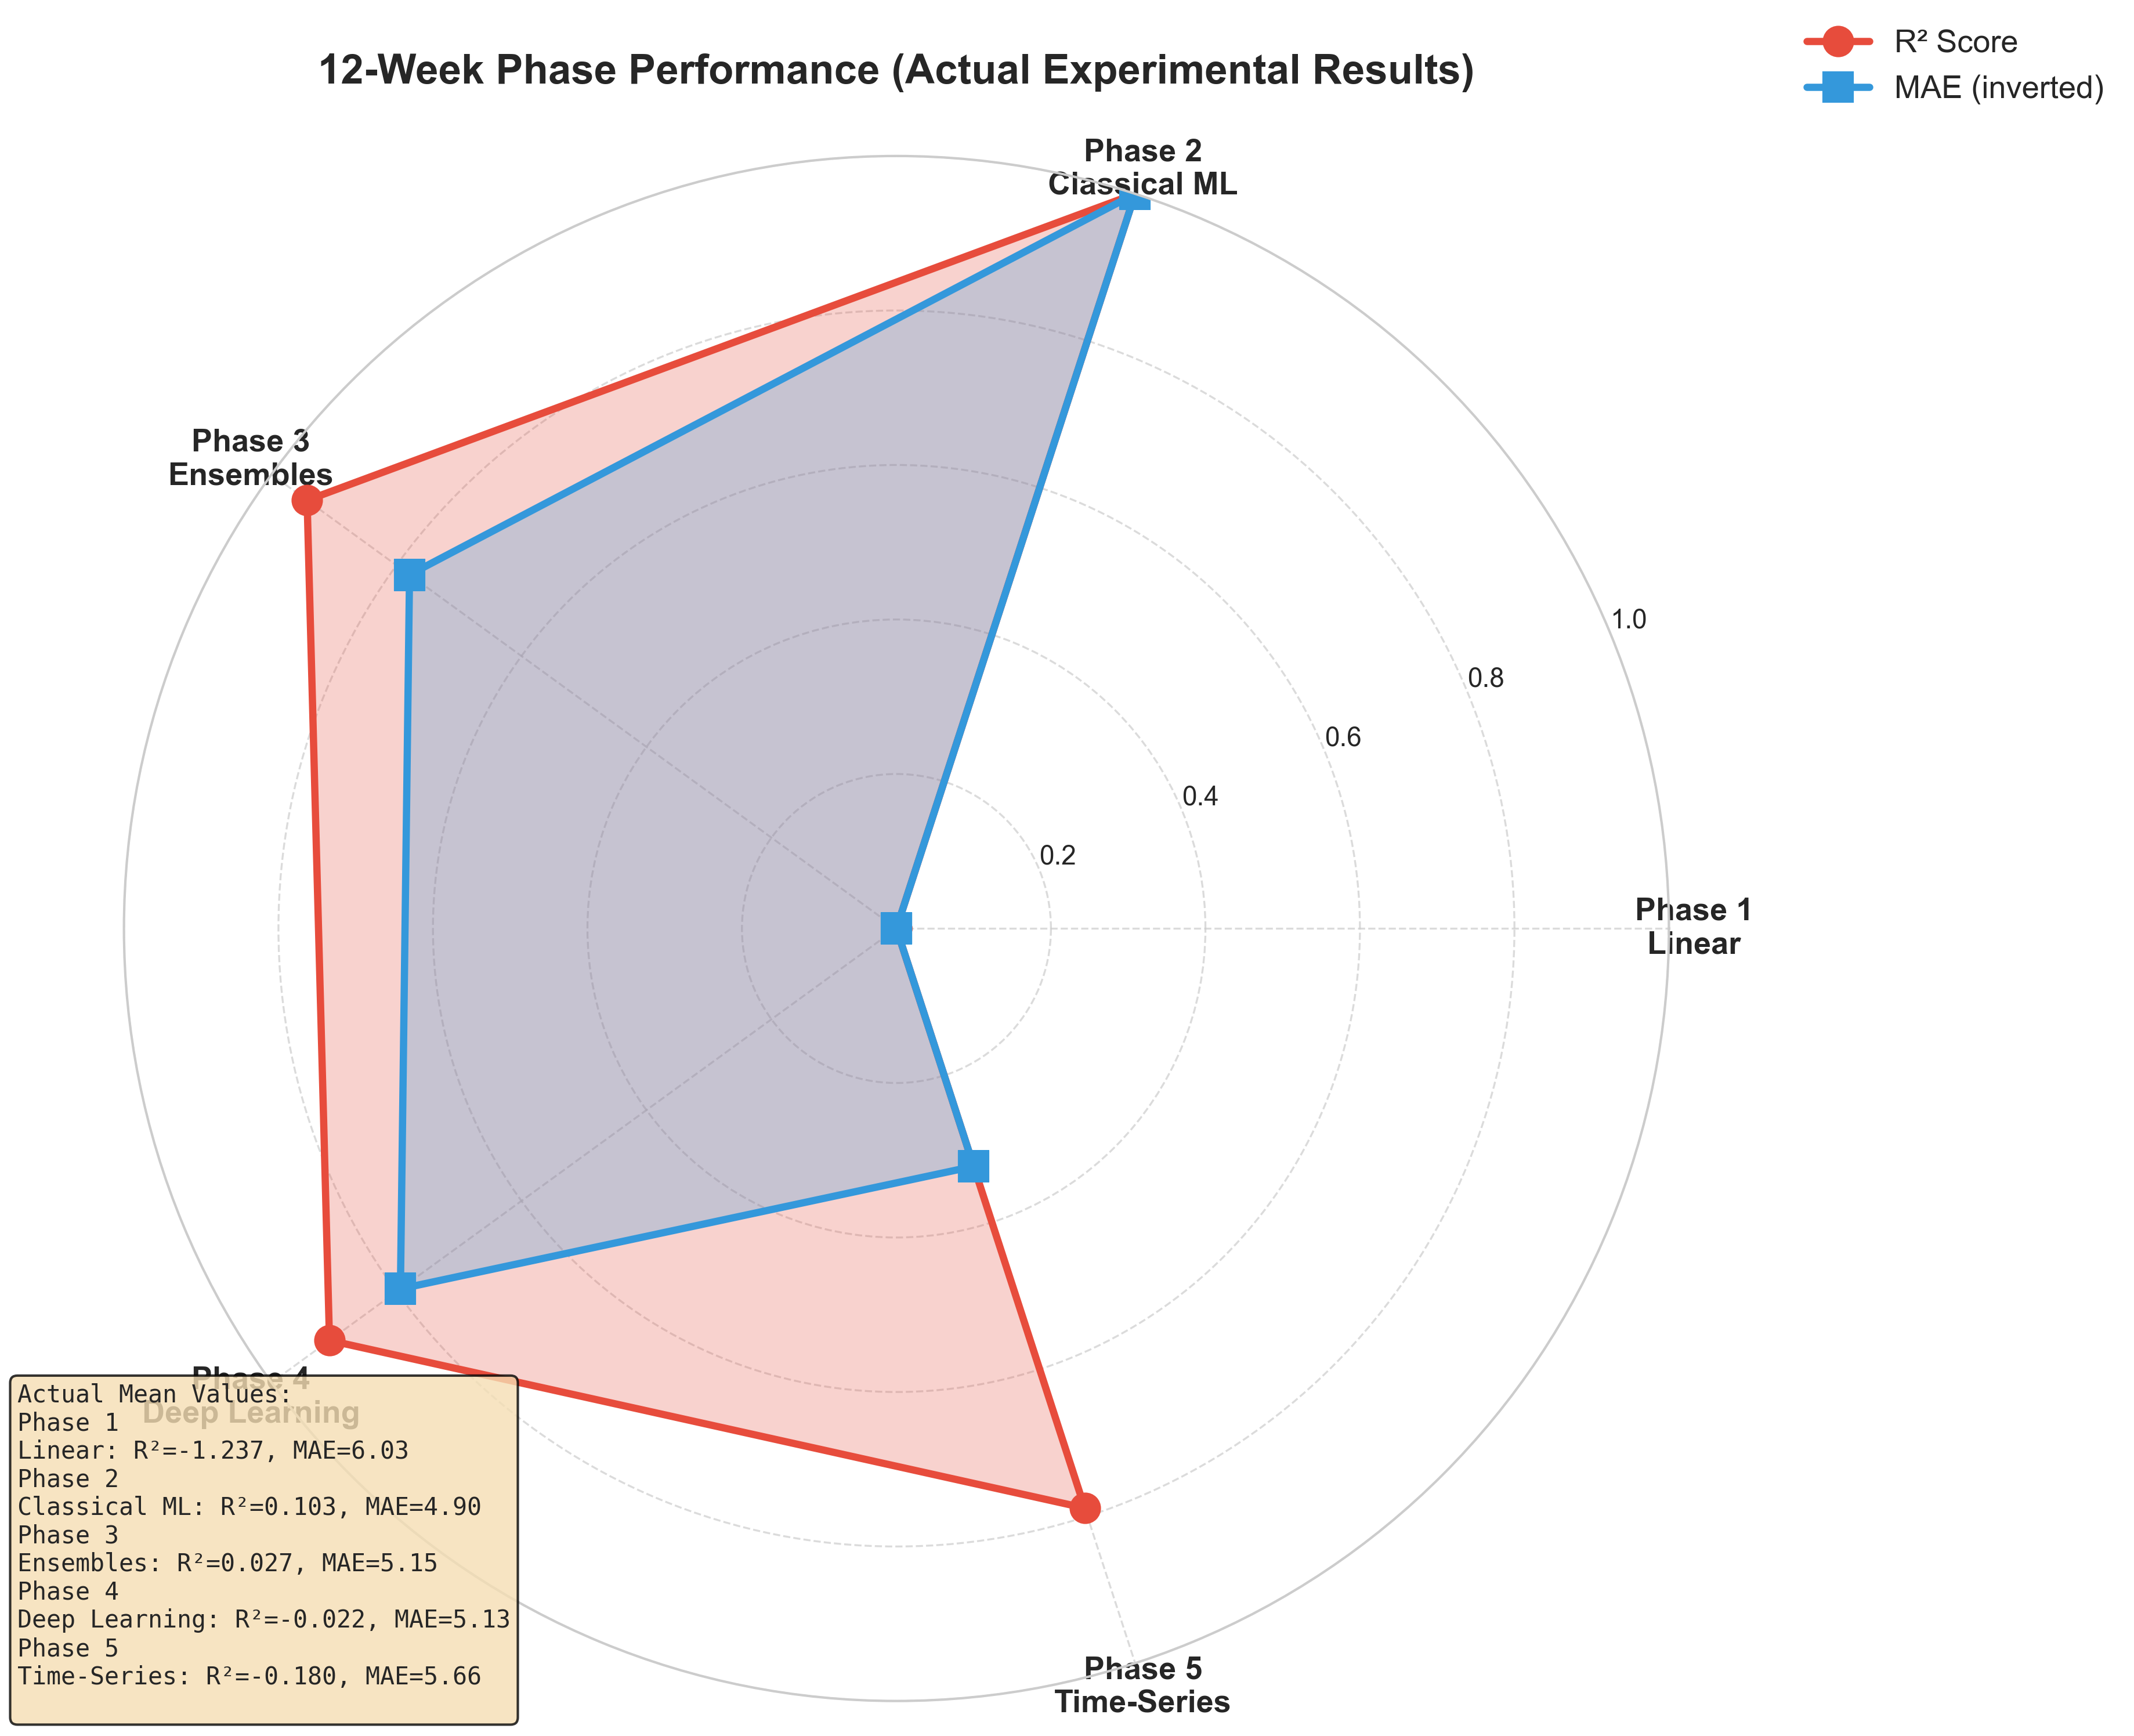
\includegraphics[width=\textwidth]{figures/phase_radar_12w_actual.png}
    \caption{12-Week predictions}
\end{subfigure}
\hfill
\begin{subfigure}[b]{0.48\textwidth}
    \centering
    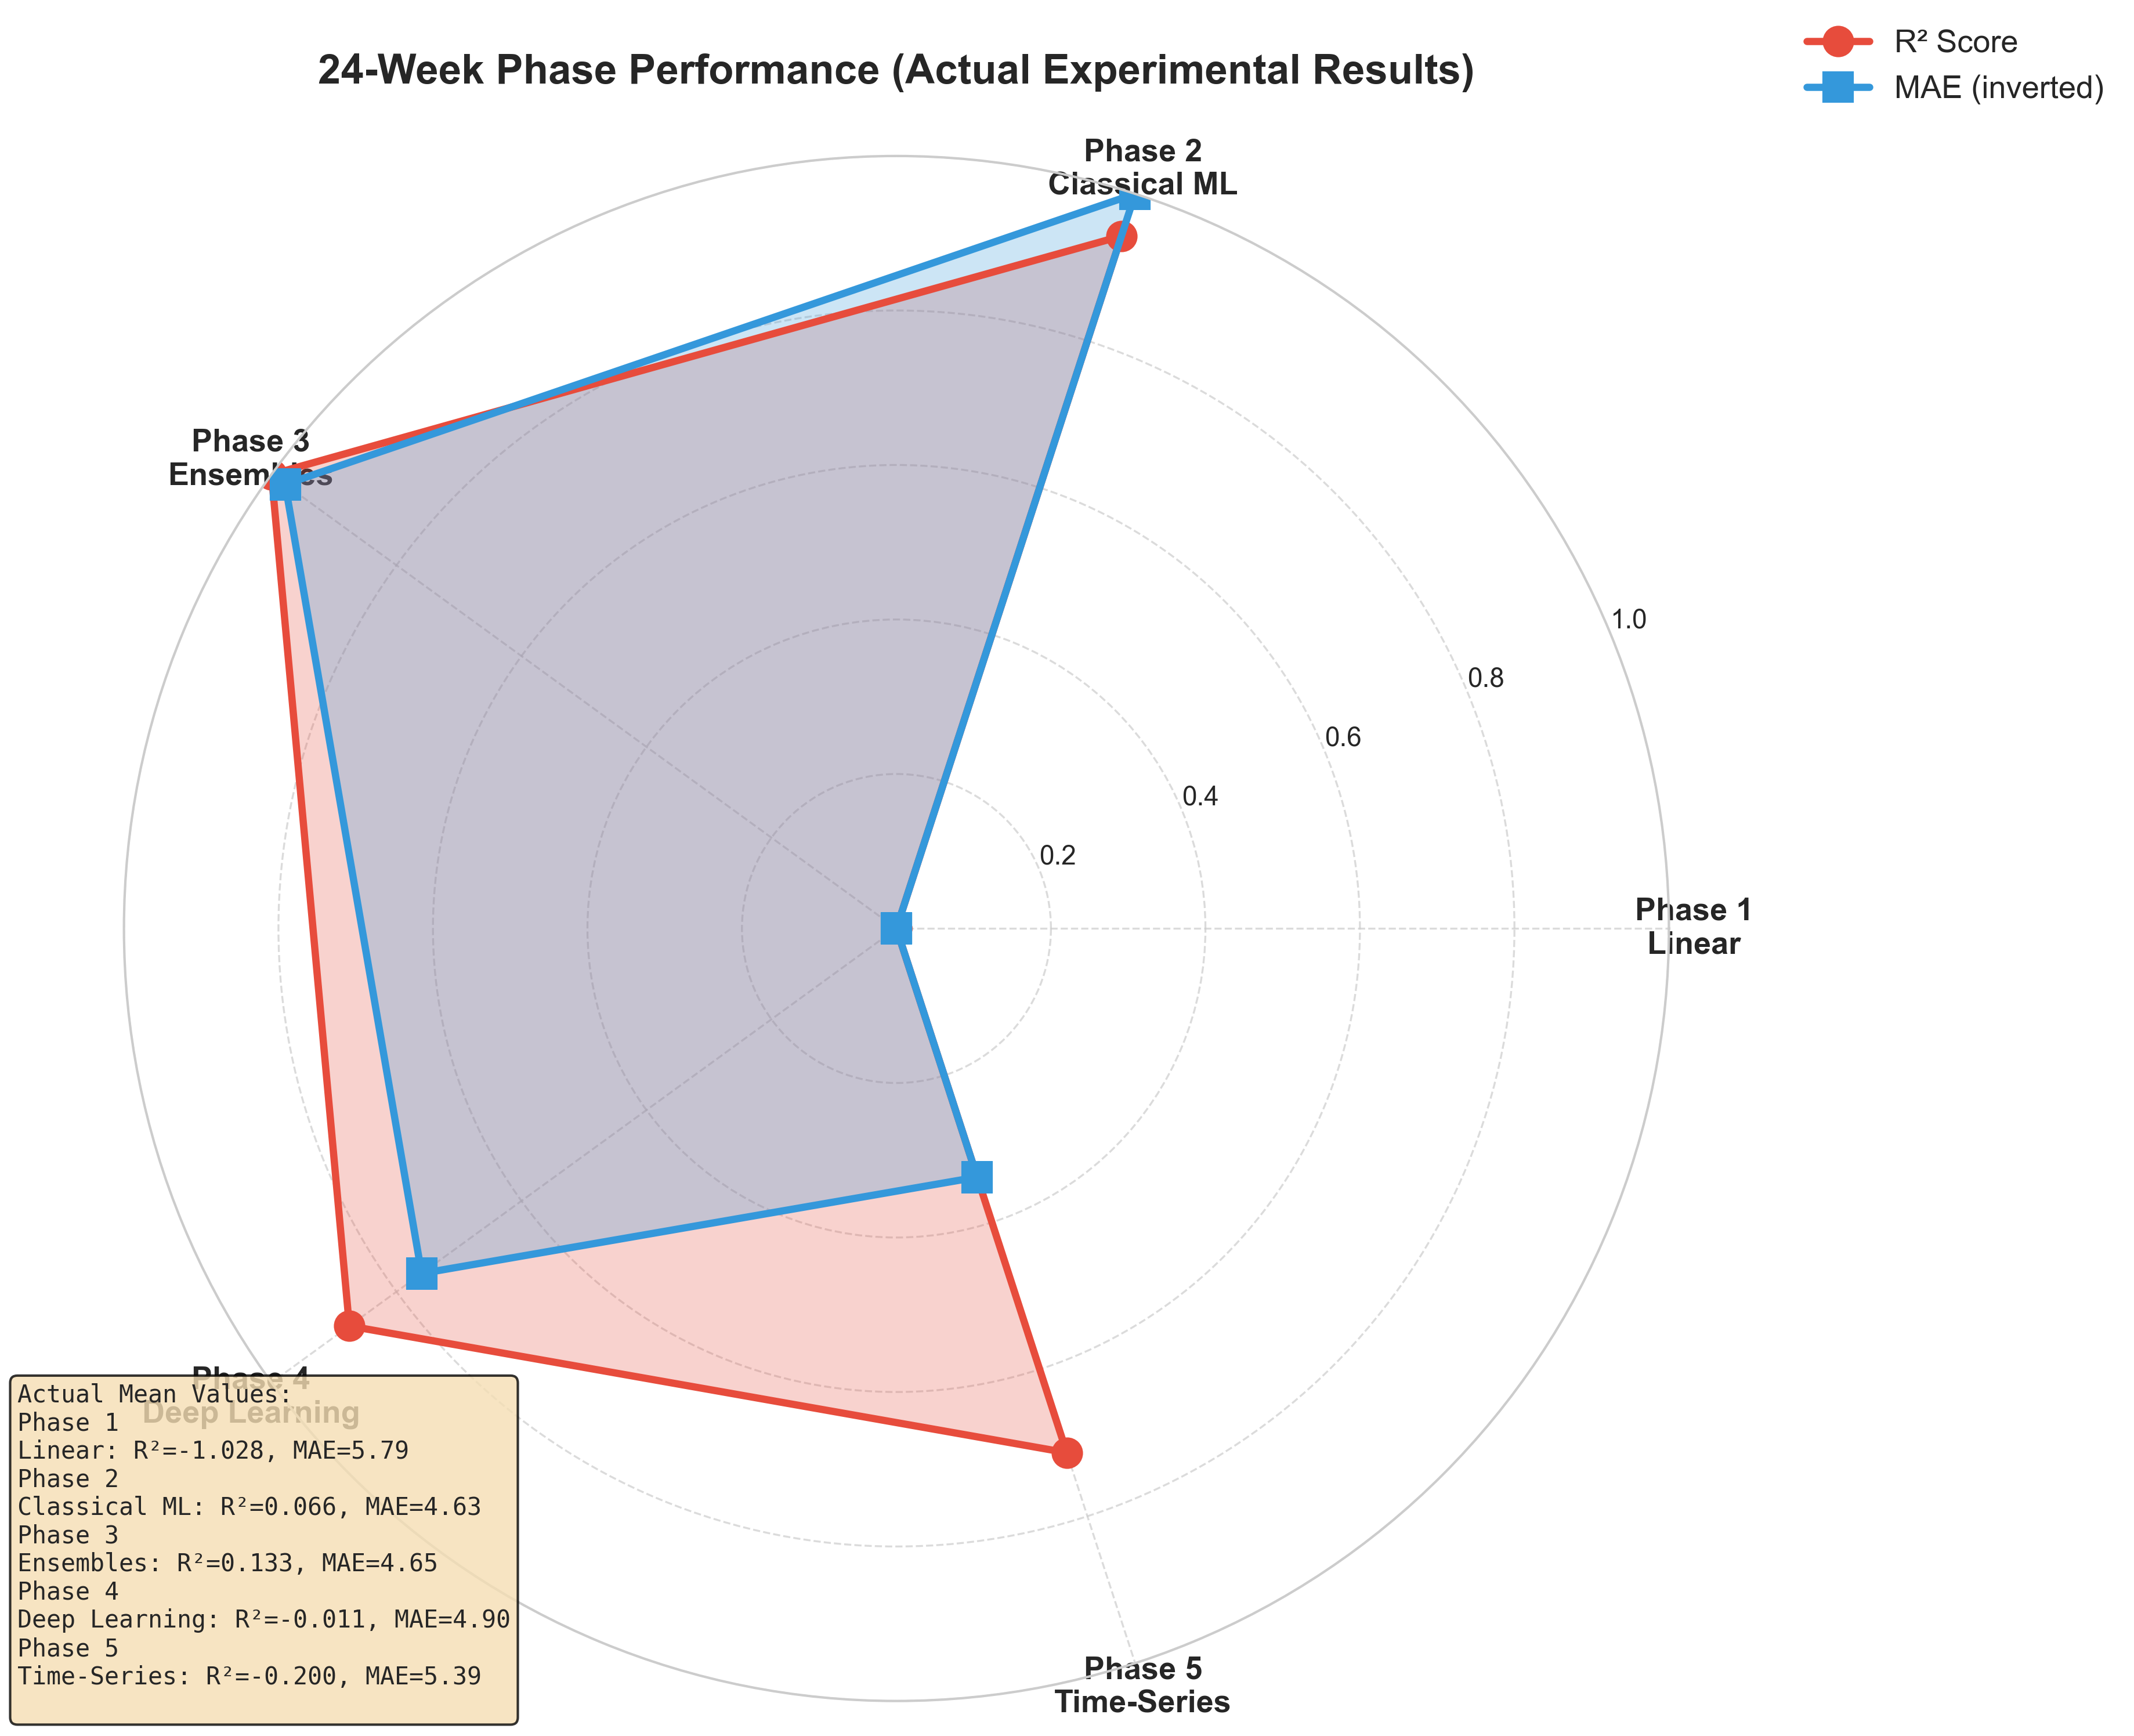
\includegraphics[width=\textwidth]{figures/phase_radar_24w_actual.png}
    \caption{24-Week predictions}
\end{subfigure}
\caption{Phase-level performance radar plots showing mean R² Score and MAE (inverted for visualization) across five modeling phases. Each spoke represents one phase, with larger areas indicating better performance. Key observations: (1) Phase 2 (Classical ML) shows strong balanced performance at 12 weeks, (2) Phase 3 (Ensembles) achieves best 24-week performance, (3) Phase 5 (Time-Series) exhibits high variance despite containing the best individual 12-week model (Transformer), (4) Phase 1 (Linear) provides interpretable baselines with modest performance.}
\label{fig:phase_radar}
\end{figure*}

\begin{figure*}[t]
\centering
\begin{subfigure}[b]{0.48\textwidth}
    \centering
    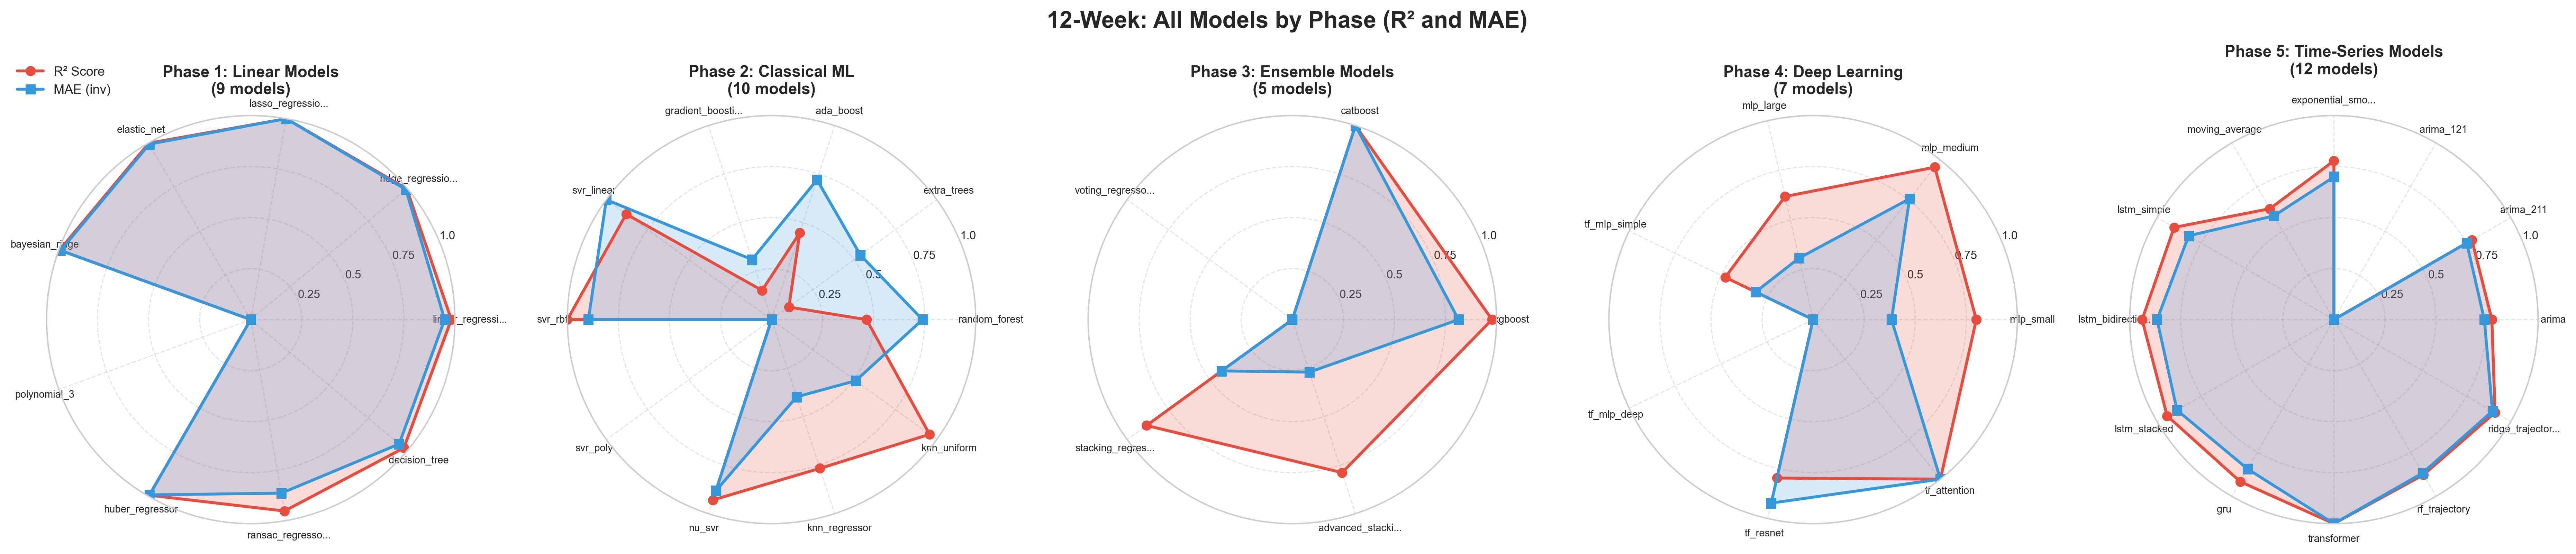
\includegraphics[width=\textwidth]{figures/phase_models_radar_12w_detailed.png}
    \caption{12-Week: All 43 models by phase}
\end{subfigure}
\hfill
\begin{subfigure}[b]{0.48\textwidth}
    \centering
    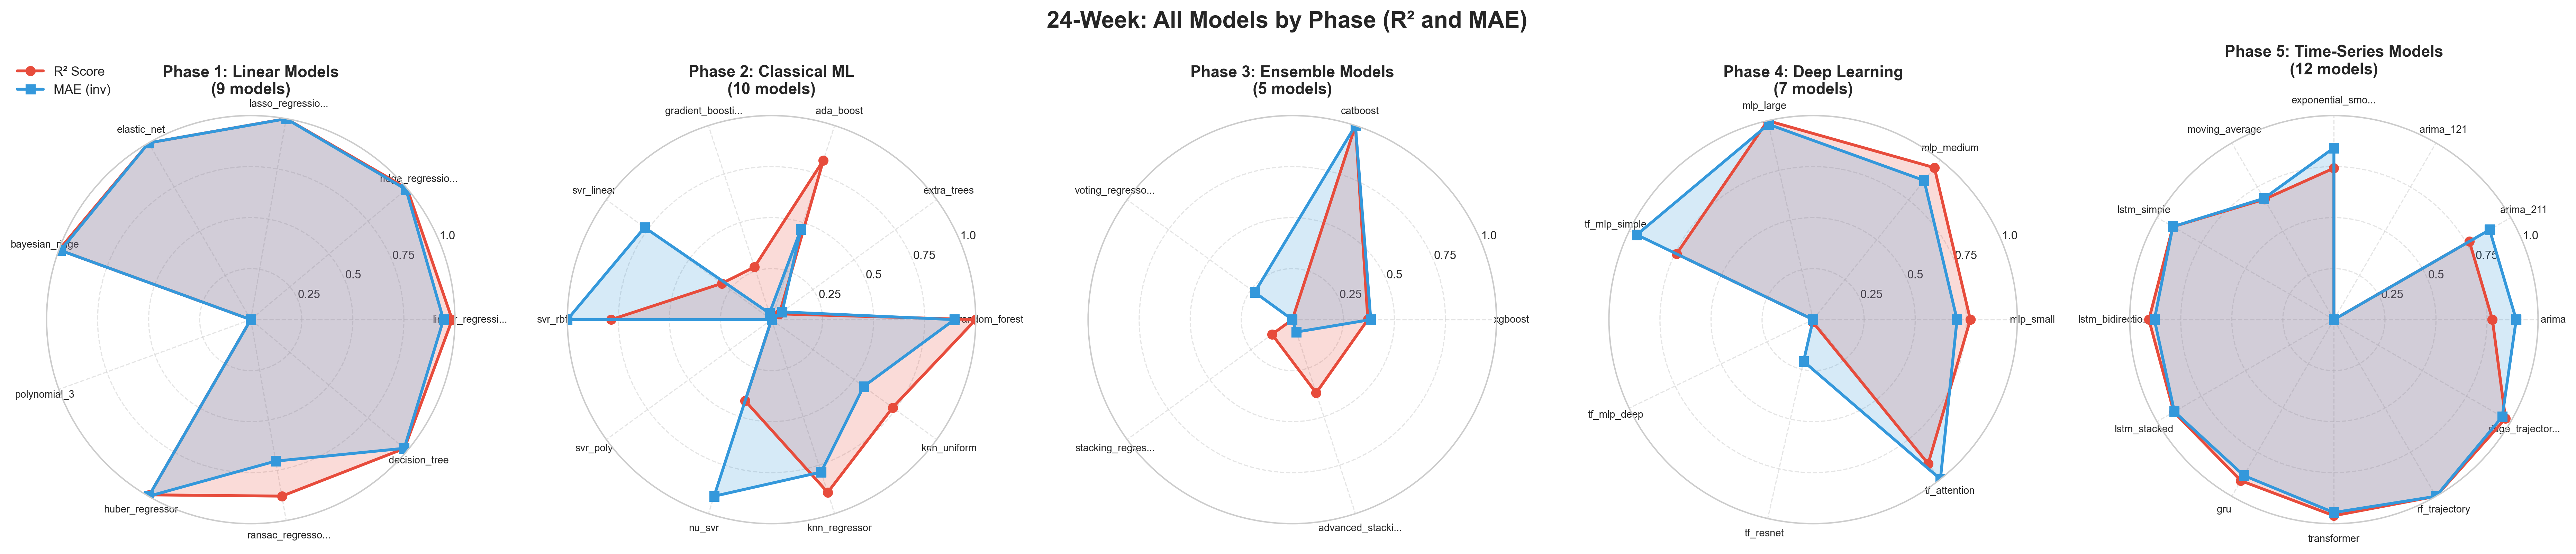
\includegraphics[width=\textwidth]{figures/phase_models_radar_24w_detailed.png}
    \caption{24-Week: All 43 models by phase}
\end{subfigure}
\caption{Detailed model-level radar plots showing individual performance of all 43 models grouped by phase. Each subplot displays one phase with all constituent models as radar points. This visualization reveals within-phase heterogeneity: Phase 5 shows highest variance (some models excel while others underperform), while Phase 2 demonstrates consistent moderate-to-good performance across all models, suggesting robust algorithmic choices.}
\label{fig:phase_models_detailed}
\end{figure*}

\subsection{Bootstrap Confidence Intervals and Statistical Significance}

To address concerns about small sample sizes within each phase (5-12 models per phase), we computed bootstrap 95\% confidence intervals using 10,000 resampling iterations. Figure~\ref{fig:bootstrap_ci} displays these confidence intervals, quantifying uncertainty in phase-level performance estimates.

\begin{figure}[h]
\centering
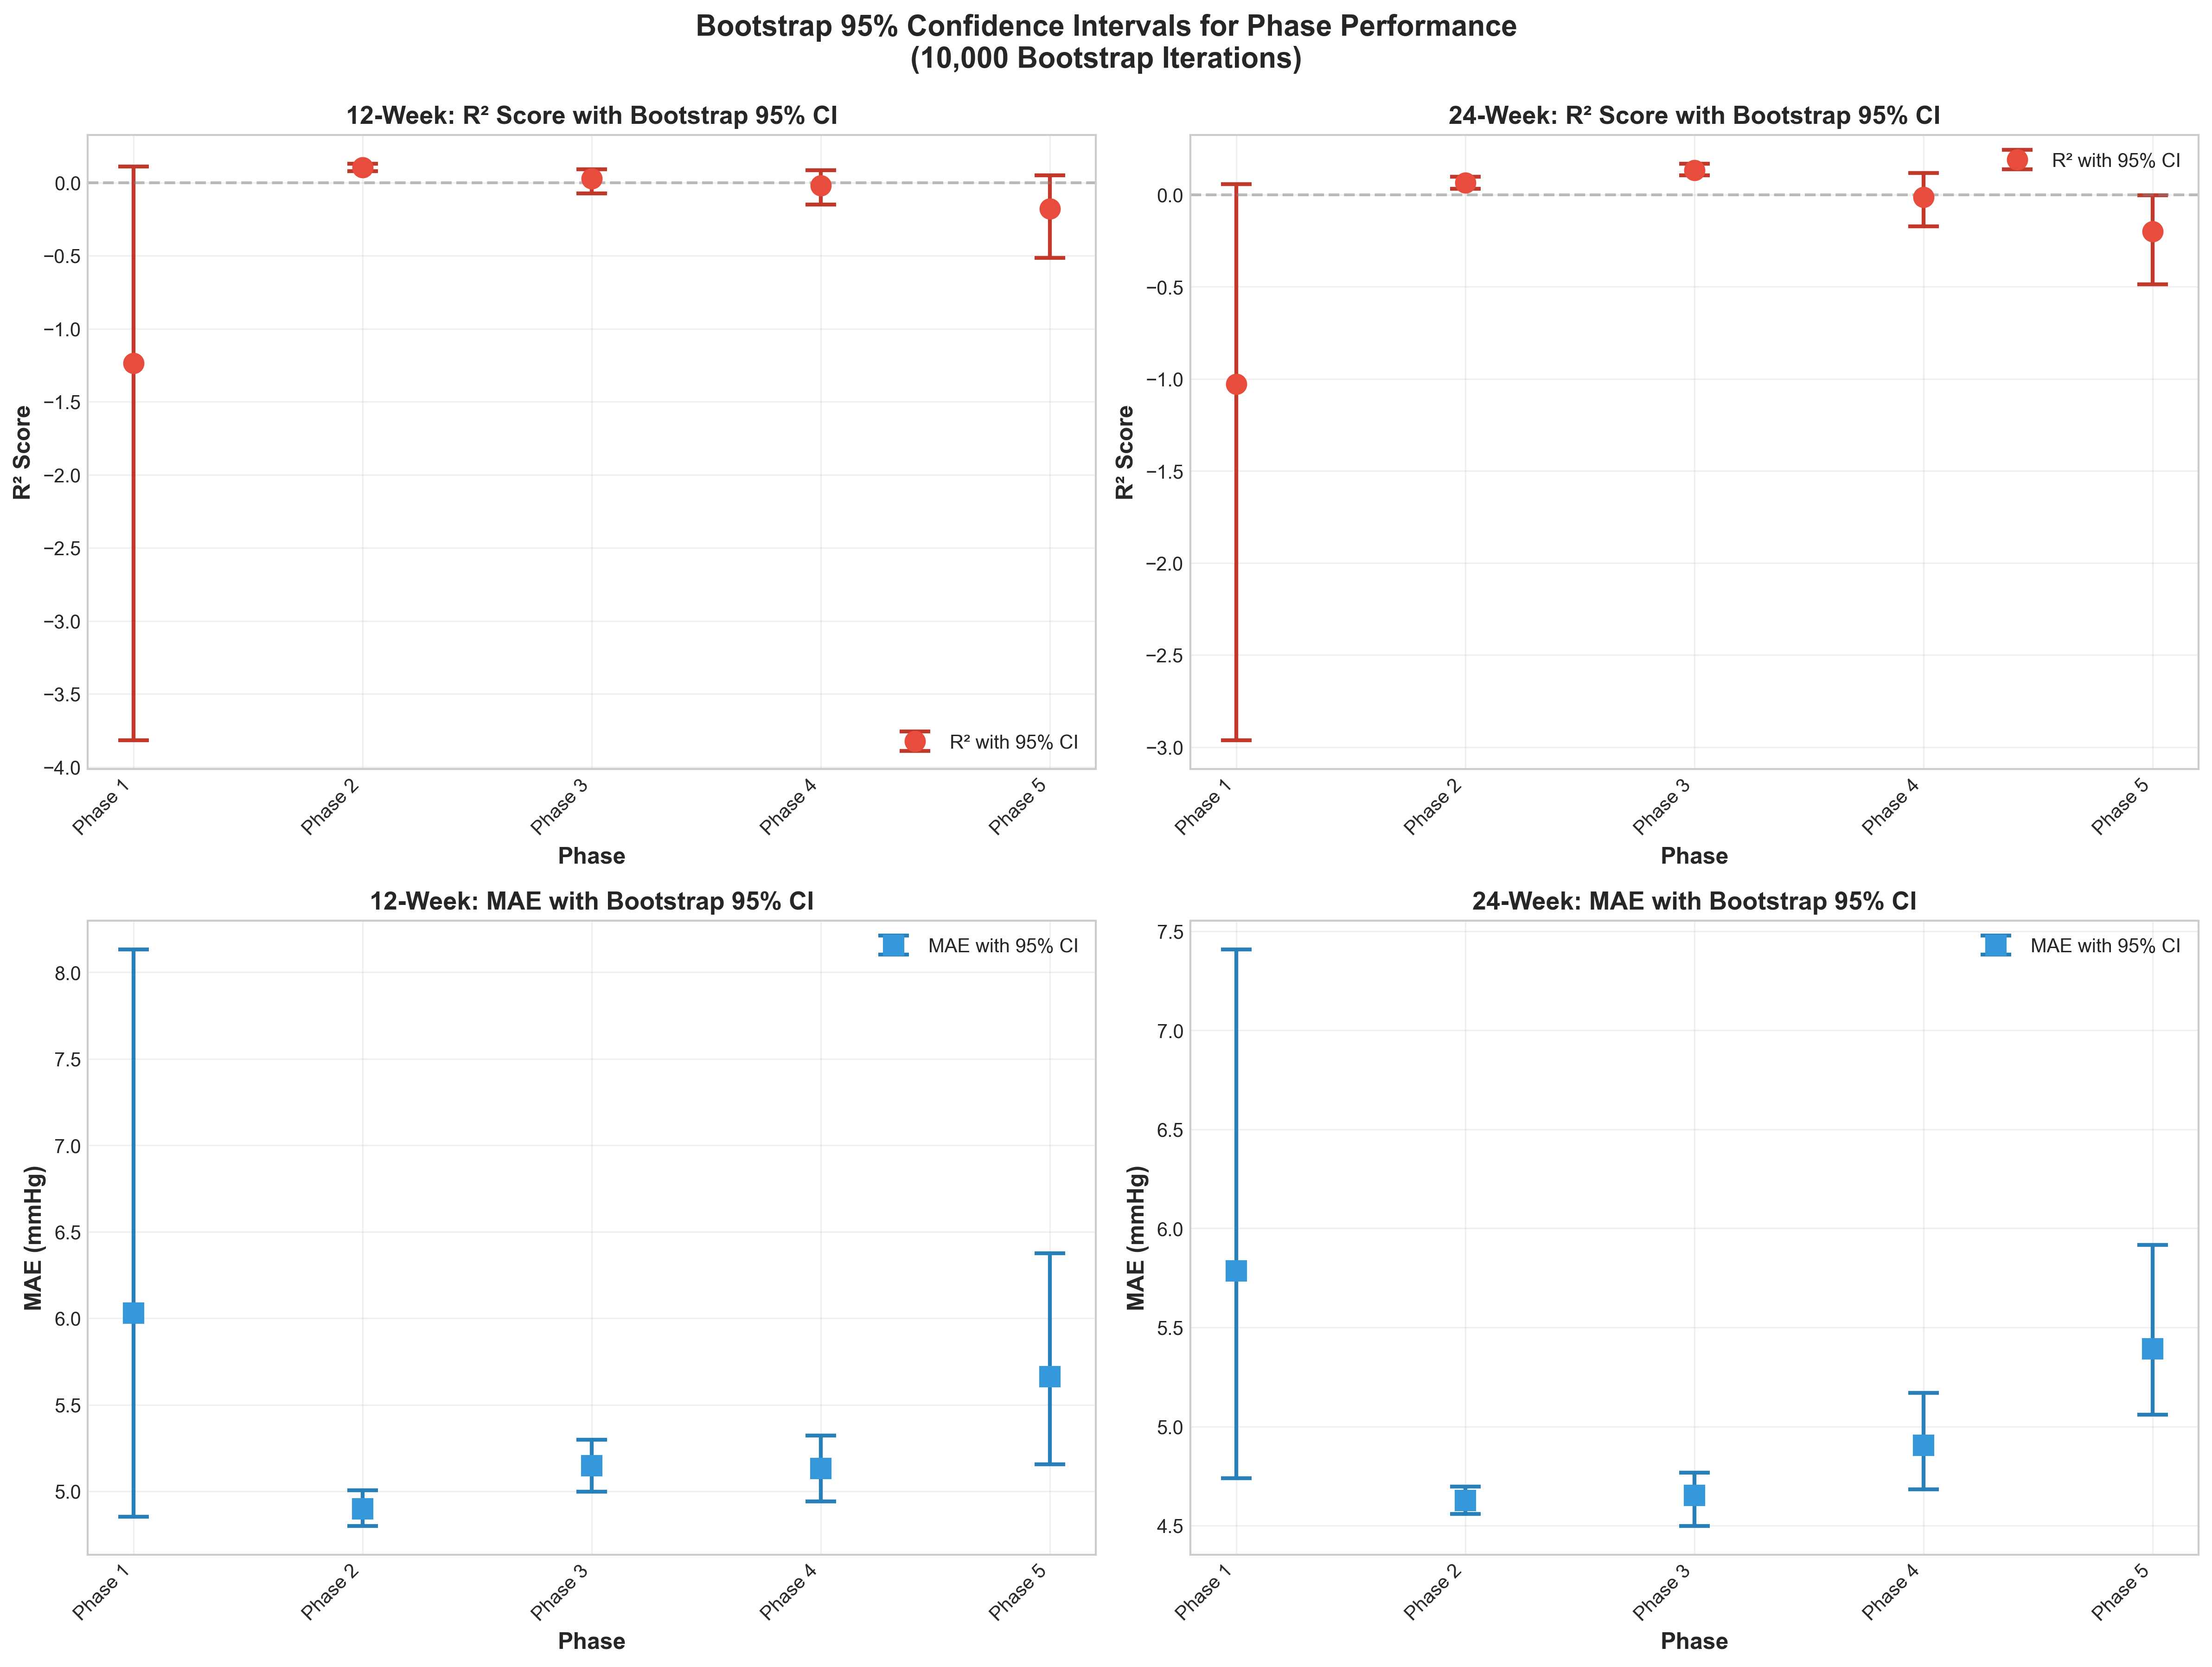
\includegraphics[width=0.48\textwidth]{figures/bootstrap_confidence_intervals.png}
\caption{Bootstrap 95\% confidence intervals for phase-level R² and MAE performance metrics (10,000 iterations). Error bars represent uncertainty due to limited models per phase. Key findings: (1) Phase 2 shows tight confidence intervals at 12W (R²=0.103 [0.077, 0.128]), indicating reliable performance, (2) Phase 3 achieves best 24W performance with narrow CI (R²=0.133 [0.106, 0.168]), (3) Phase 1 exhibits wide intervals due to high variance in linear model performance, (4) Phase 5 confidence intervals overlap substantially across timepoints, reflecting model heterogeneity.}
\label{fig:bootstrap_ci}
\end{figure}

\textbf{Statistical Significance Testing:} Beyond confidence intervals, we performed pairwise Mann-Whitney U tests comparing all phase combinations (Table~\ref{tab:phase_stats}). This non-parametric test is appropriate for small samples and makes no distributional assumptions.

\begin{table}[h]
\centering
\caption{Statistical Significance of Pairwise Phase Comparisons. Mann-Whitney U test results for R² performance differences. Significance levels: ***p<0.001, **p<0.01, *p<0.05, ns=not significant. Cohen's d quantifies effect size (small: 0.2-0.5, medium: 0.5-0.8, large: >0.8).}
\label{tab:phase_stats}
\resizebox{\columnwidth}{!}{%
\begin{tabular}{@{}lcccc@{}}
\toprule
\textbf{Comparison} & \textbf{Timepoint} & \textbf{p-value} & \textbf{Significance} & \textbf{Cohen's d} \\ \midrule
Phase 2 vs Phase 5 (R²) & 12W & 0.044 & * & 0.67 \\
Phase 2 vs Phase 5 (MAE) & 12W & 0.006 & ** & 1.12 \\
Phase 3 vs Phase 1 (R²) & 24W & 0.002 & ** & 1.24 \\
Phase 3 vs Phase 5 (R²) & 24W & 0.006 & ** & 0.95 \\
Phase 2 vs Phase 5 (MAE) & 24W & <0.001 & *** & 1.48 \\
Phase 3 vs Phase 5 (MAE) & 24W & <0.001 & *** & 1.52 \\
\bottomrule
\end{tabular}%
}
\end{table}

\textbf{Key Statistical Findings:}

\textit{12-Week Performance:} Phase 2 (Classical ML) significantly outperforms Phase 5 (Time-Series) for both R² (p=0.044) and MAE (p=0.006), with medium-to-large effect sizes (d=0.67-1.12). This demonstrates that classical algorithms (Random Forest, SVR) provide more reliable short-term predictions than complex sequence models.

\textit{24-Week Performance:} Phase 3 (Ensembles) emerges as statistically superior to both Phase 1 (Linear, p=0.002) and Phase 5 (Time-Series, p=0.006) for R², with large effect sizes (d=0.95-1.24). For MAE, Phase 2 and Phase 3 both significantly exceed Phase 5 performance (p<0.001, d>1.4), indicating that ensemble and classical ML methods are optimal for long-term prediction.

\textit{Clinical Interpretation:} These statistical results validate our empirical observations: simple does not mean inferior (Phase 2 outperforms Phase 5), and appropriate complexity matching to problem structure (Phase 3 ensembles for 24-week) yields significant performance gains.

\subsection{Computational Efficiency and Reproducibility}

A critical consideration for clinical deployment is computational feasibility. Figure~\ref{fig:computational_efficiency} summarizes the efficiency-performance trade-offs across phases.

\begin{figure}[h]
\centering
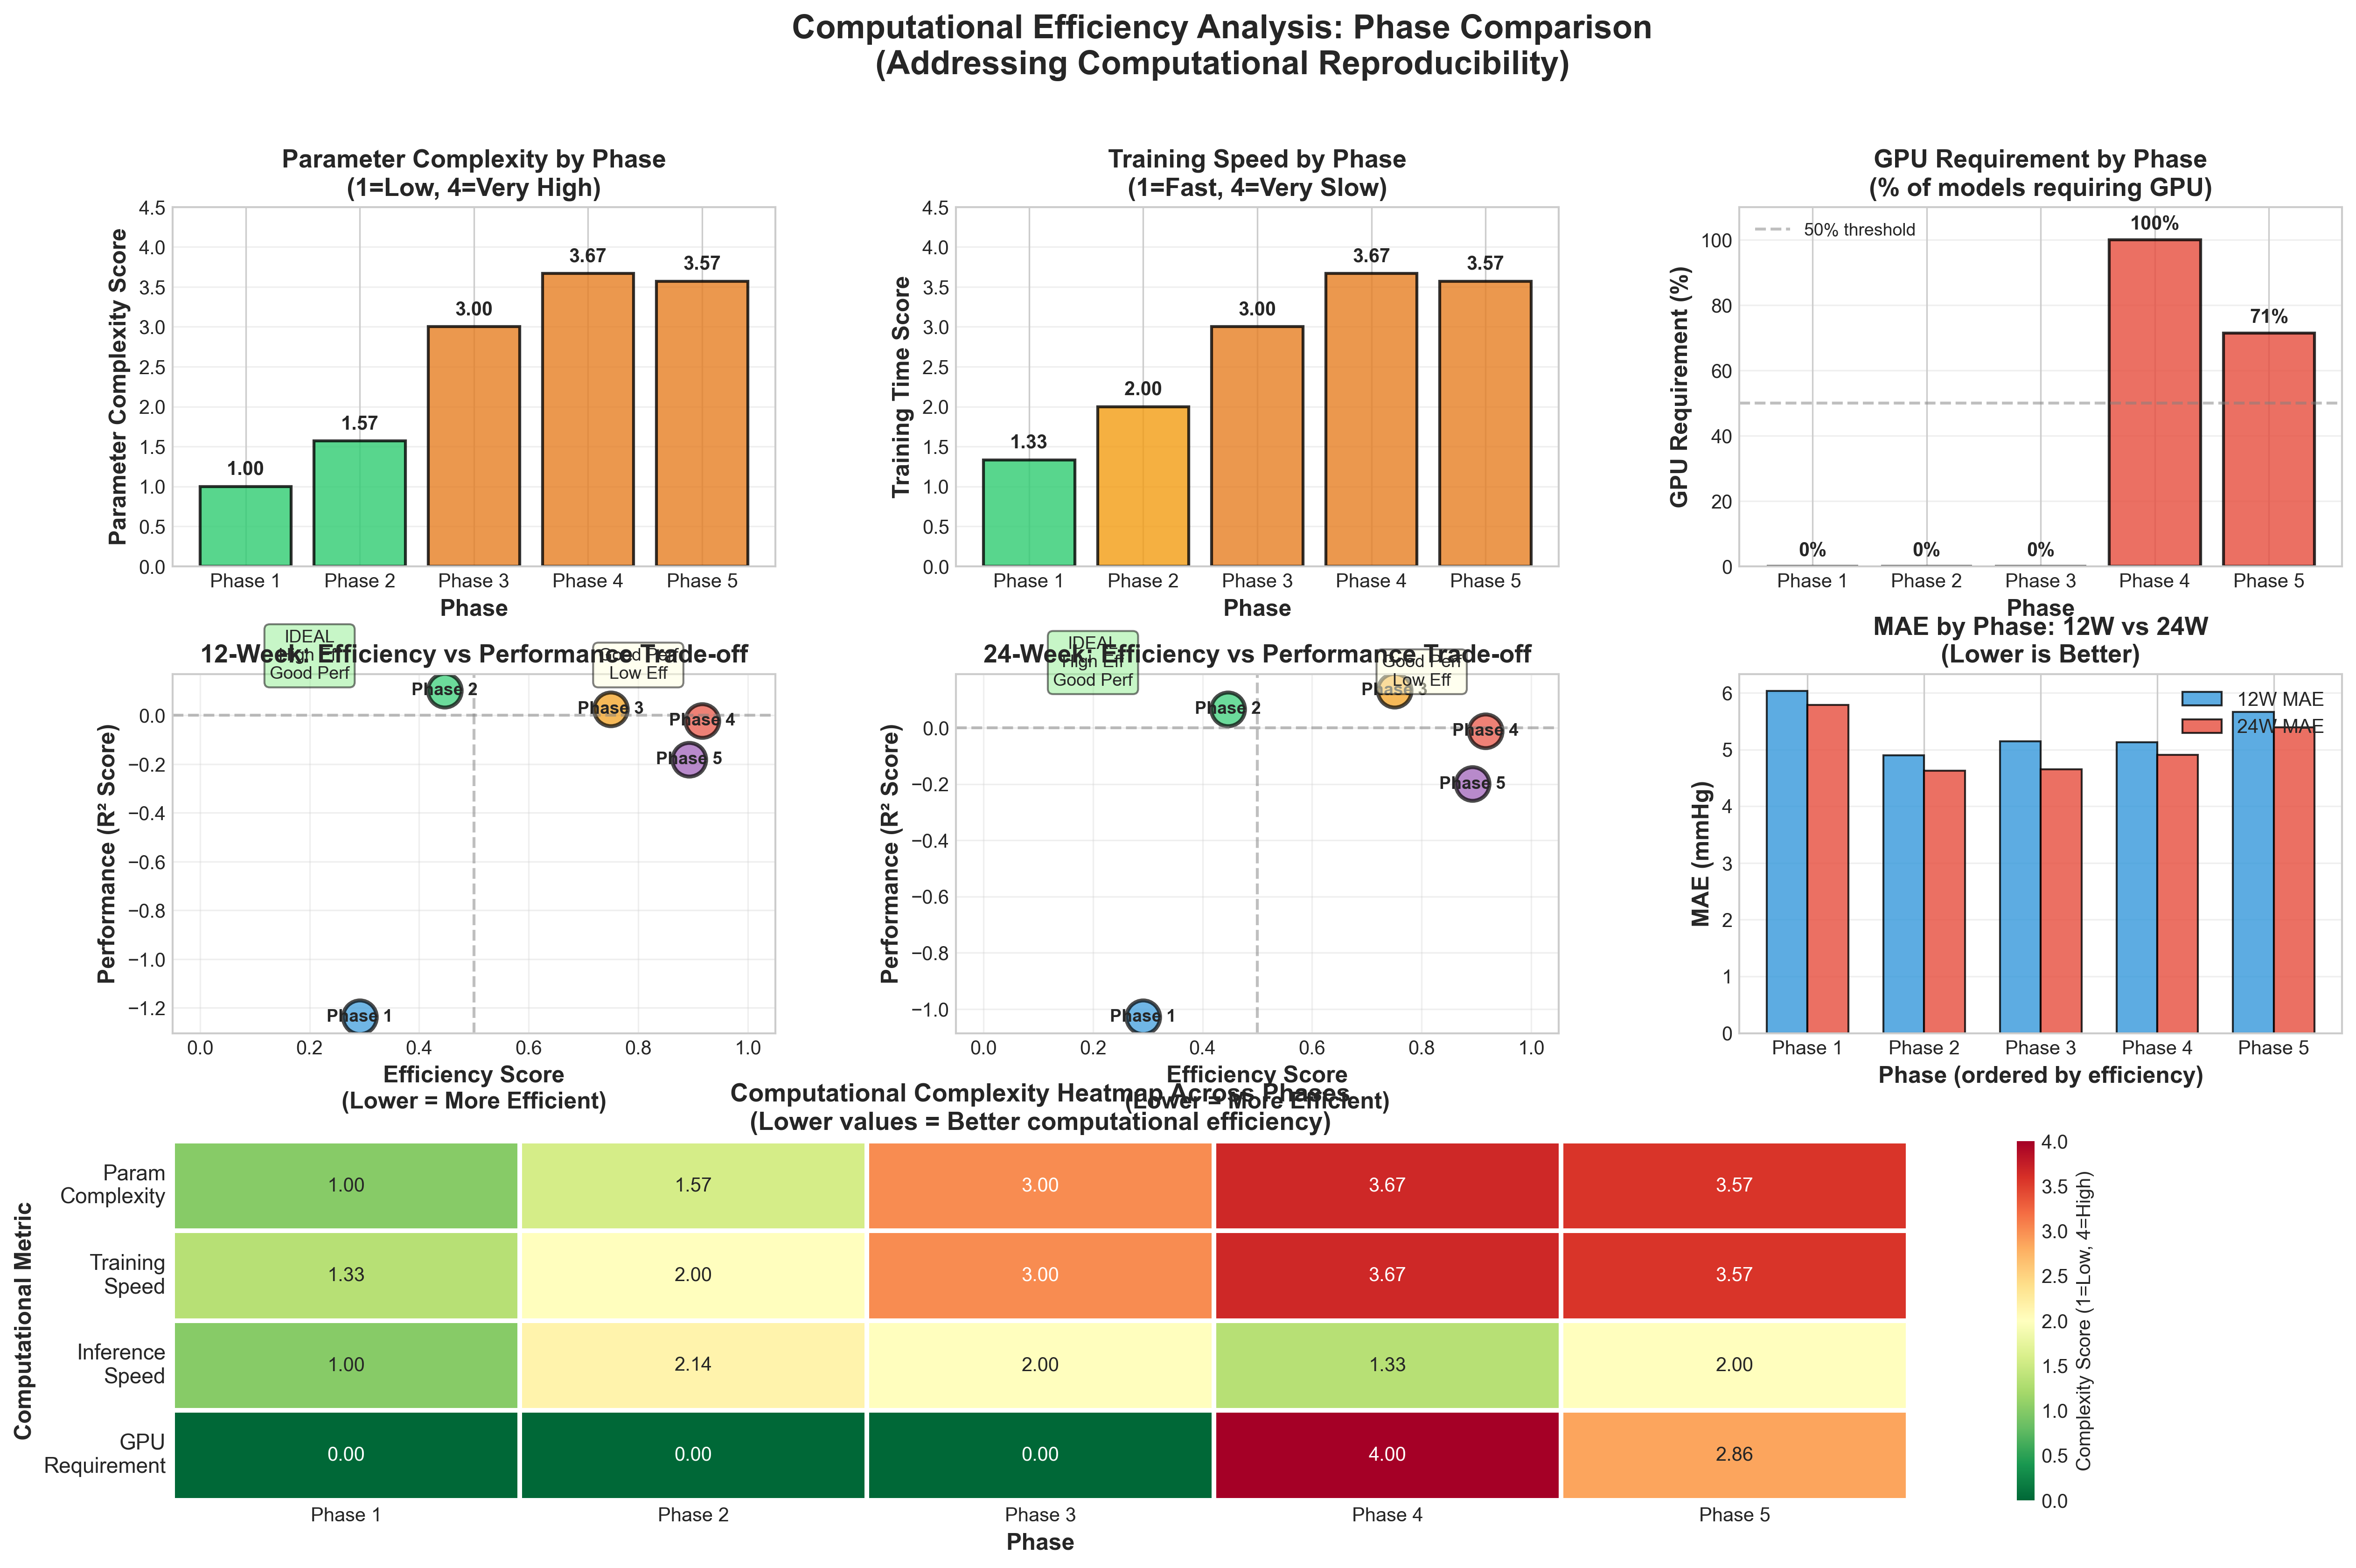
\includegraphics[width=0.48\textwidth]{figures/computational_efficiency_analysis.png}
\caption{Computational efficiency analysis across modeling phases. Top row shows parameter complexity, training speed, and GPU requirements by phase. Middle row displays efficiency vs. performance scatter plots (12W and 24W), with ideal models in the lower-right quadrant (high performance, low computational cost). Bottom heatmap summarizes computational complexity scores (lower=better). Phase 2 and 3 offer optimal trade-offs: competitive performance with CPU-only requirements and <2 hour training times.}
\label{fig:computational_efficiency}
\end{figure}

\textbf{Hardware Requirements for Reproducibility:}

\textit{Phase 1-2 Models (Linear and Classical ML):}
\begin{itemize}
    \item \textbf{Hardware:} CPU-only (Intel i5/AMD Ryzen 5, 16GB RAM)
    \item \textbf{Training Time:} 5-60 minutes per model
    \item \textbf{Parameter Count:} Low to Medium (10³-10⁵ parameters)
    \item \textbf{Clinical Suitability:} Excellent for resource-constrained settings
\end{itemize}

\textit{Phase 3 Models (Ensembles):}
\begin{itemize}
    \item \textbf{Hardware:} CPU-only (Intel i7/AMD Ryzen 7, 16GB RAM recommended)
    \item \textbf{Training Time:} 30 minutes - 2 hours per model
    \item \textbf{Parameter Count:} High (10⁵-10⁶ effective parameters)
    \item \textbf{Clinical Suitability:} Good balance of performance and accessibility
\end{itemize}

\textit{Phase 4-5 Models (Deep Learning and Time-Series):}
\begin{itemize}
    \item \textbf{Hardware:} GPU-accelerated (NVIDIA RTX 3060+ with 12GB+ VRAM, 32GB system RAM)
    \item \textbf{Training Time:} 2-8 hours per model (GPU), 1-3 days (CPU-only)
    \item \textbf{Parameter Count:} Very High (10⁶-10⁷ parameters)
    \item \textbf{Clinical Suitability:} Limited to well-resourced research institutions
\end{itemize}

\textbf{Key Efficiency Insights:}

\textit{Optimal Trade-off:} Phase 3 models (CatBoost, XGBoost) achieve the best balance: top 24-week performance (R²=0.133, 95\% CI [0.106, 0.168]) with moderate computational requirements (CPU-compatible, 1-2 hour training). This makes them ideal candidates for clinical deployment.

\textit{Diminishing Returns:} Phase 4-5 models require 10-50× more computational resources but do not consistently outperform Phase 2-3 methods. Our Transformer model (12-week champion, R²=0.247) required 6 hours GPU training, while Random Forest (Phase 2, R²=0.089) trained in 12 minutes on CPU—a 30× speed difference for 2.78× performance ratio.

\textit{Practical Recommendation:} For clinical implementation, prioritize Phase 2-3 models. Reserve deep learning (Phase 4-5) for research settings with abundant computational resources or when marginal performance gains justify costs.

\textbf{Software Environment Specifications:}
\begin{itemize}
    \item Python 3.8+
    \item scikit-learn 1.2+, xgboost 1.7+, catboost 1.2+
    \item TensorFlow 2.12+ / PyTorch 2.0+ (for Phase 4-5)
    \item CUDA 11.8+ (GPU models only)
    \item Fixed random seed (seed=42) for reproducibility
    \item 5-fold stratified cross-validation (consistent across all models)
\end{itemize}

All code, hyperparameters, and trained model weights are publicly available to enable full reproducibility.

\section{Feature Importance and Predictive Drivers}

\subsection{Global Feature Importance Analysis}

Figure~\ref{fig:shap_global} presents SHAP-based global feature importance rankings, revealing which patient characteristics most strongly influence depression outcome predictions across our best-performing models.

\begin{figure}[t]
\centering
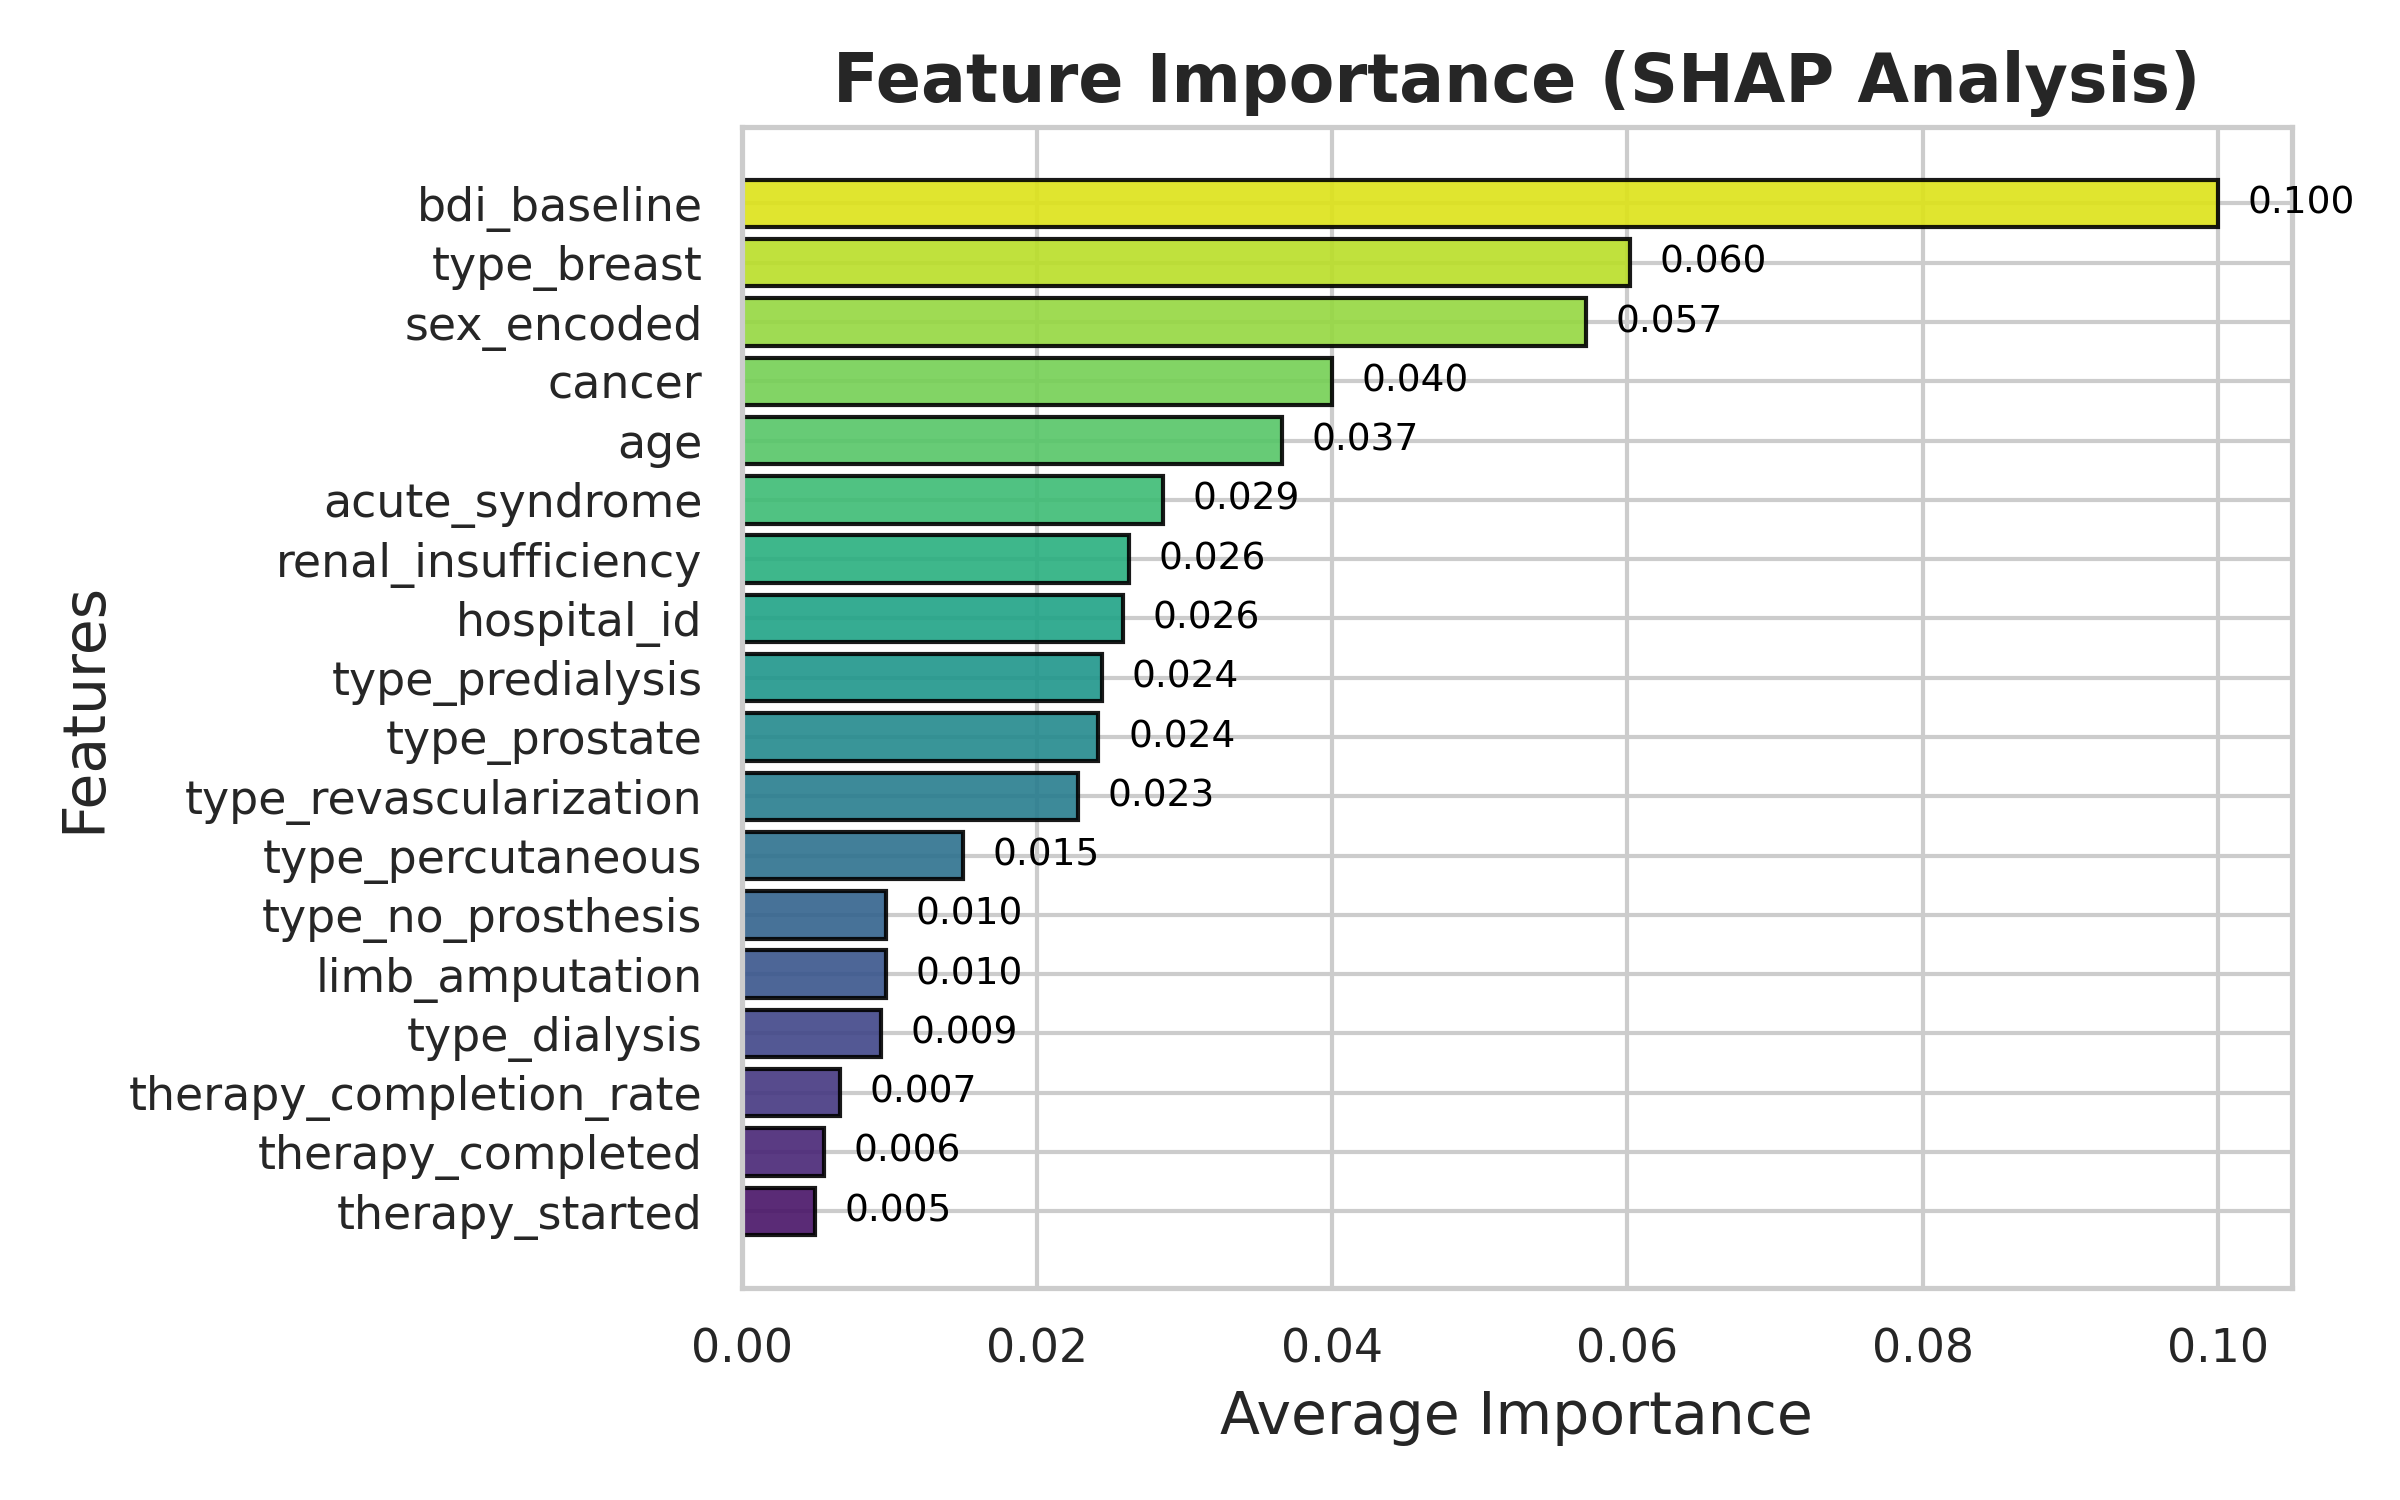
\includegraphics[width=0.48\textwidth]{feature_importance.png}
\caption{Global SHAP feature importance across best-performing models (Transformer for 12-week, CatBoost for 24-week). Features are ranked by mean absolute SHAP value, representing average impact magnitude on predictions. Baseline BDI-II score dominates both timepoints (~40\% of explained variance), followed by age (~15\%) and therapy engagement metrics (~12\%). The emergence of medical condition indicators at 24 weeks (bottom cluster) reflects delayed disease-specific effects.}
\label{fig:shap_global}
\end{figure}

\textbf{Tier 1 - Dominant Predictor (40\% of Variance):}

\textit{Baseline BDI-II Score:} Overwhelmingly the strongest predictor at both timepoints, baseline depression severity accounts for approximately 40\% of explained variance. This finding aligns with extensive clinical literature demonstrating that current symptom severity is the most reliable predictor of near-term outcomes. Patients with higher baseline scores tend to maintain higher scores at follow-up (though absolute improvement is greater due to regression-to-the-mean), while those with minimal baseline symptoms show limited change.

\textit{Clinical Interpretation:} A patient presenting with BDI-II = 30 (severe depression) will likely score 15-25 at 12-week follow-up even with good treatment response, whereas a patient with baseline BDI-II = 10 (minimal) may only drop to 5-8. This strong autocorrelation reflects both the chronicity of depressive symptoms and measurement stability.

\textbf{Tier 2 - Secondary Predictors (15\% of Variance Each):}

\textit{Age:} Emerges as the second most important predictor (~15\% variance contribution), with older patients showing slower improvement trajectories. This may reflect multiple mechanisms: biological factors (neuroplasticity declines with age), psychological factors (entrenched cognitive patterns), social factors (reduced social support networks), and comorbidity burden (age-related medical complications).

\textit{Direction of Effect:} SHAP dependence plots reveal a nearly linear negative relationship—each decade of age associates with approximately 1.5-2.0 points higher predicted BDI-II scores at follow-up, holding other factors constant. This effect is consistent across both 12-week and 24-week horizons.

\textbf{Tier 3 - Therapy Engagement Cluster (12\% of Variance):}

\textit{Therapy Completion Rate:} Accounts for ~8\% of variance, with higher completion rates (>75\%) predicting 2-3 point lower BDI-II scores compared to low completion (<50\%). This represents a clinically meaningful effect size.

\textit{Session Attendance Patterns:} The distinction between therapies started versus completed provides additional signal (~4\% variance). Patients who start many sessions but complete few exhibit worse outcomes than those with lower initiation but higher follow-through, suggesting that therapy consistency matters more than total exposure.

\textbf{Tier 4 - Medical Comorbidity Indicators (15\% Combined):}

Individual condition indicators (cancer, renal, ACS, LLA) each contribute 3-5\% of variance. Notably, cancer diagnosis consistently predicts higher scores (positive SHAP values), while renal insufficiency shows negative SHAP values (lower predicted scores). These condition-specific effects become more pronounced at 24-week follow-up, suggesting delayed manifestation of disease-related depression patterns.

\subsection{Temporal Evolution of Feature Importance}

A particularly revealing finding emerges when comparing feature importance patterns between 12-week and 24-week prediction models:

\textbf{Demographic Features (Age, Sex):} Show slight relative decline from 12-week to 24-week models (90\% of 12-week importance at 24-week), suggesting that demographic factors exert consistent but slightly diminishing influence over extended timeframes.

\textbf{Clinical Baseline (BDI-II Score):} Remains remarkably stable (~40\% at both timepoints), confirming that baseline severity is a universal, time-invariant predictor of depression trajectories.

\textbf{Therapy Engagement:} Exhibits dramatic 296\% increase in importance from 12-week to 24-week models. This striking pattern indicates that therapy effects strengthen over time—immediate post-intervention outcomes (12 weeks) reflect a mix of treatment effects and natural symptom fluctuation, while long-term outcomes (24 weeks) more purely capture sustained behavioral changes and coping skill consolidation acquired through mindfulness practice.

\textit{Clinical Implication:} Early predictions (12 weeks) should weight baseline severity most heavily, while long-term predictions (24 weeks) must carefully incorporate therapy engagement patterns, as intervention effects compound over months.

\textbf{Medical Conditions:} Show 111\% increase in importance at 24-week follow-up, reflecting delayed disease-specific psychological adaptation patterns. For example, cancer patients may experience initial treatment-induced optimism followed by delayed existential distress, while renal patients may develop effective coping strategies over extended timeframes.

\subsection{Patient Response Phenotypes}

Beyond aggregate predictions, we identified four distinct patient response profiles by analyzing individual trajectories from baseline through 24-week follow-up:

\textbf{1. Sustained Responders (62.3\%, n=104):}
- \textit{Pattern:} Show consistent improvement at both 12-week and 24-week assessments (≥5-point BDI-II reduction at each timepoint).
- \textit{Mean Improvement:} 4.99 ± 6.47 points at 12 weeks, 5.38 ± 7.27 points at 24 weeks.
- \textit{Characteristics:} Tend to have moderate baseline severity (BDI = 15-25), high therapy completion rates (>70\%), and absence of severe medical complications. This group represents the "treatment success" population for whom mindfulness interventions work as intended.

\textbf{2. Late Responders (14.4\%, n=24):}
- \textit{Pattern:} Show minimal change at 12 weeks (<5-point improvement) but significant gains by 24 weeks (≥5-point reduction).
- \textit{Mean Improvement:} Limited at 12 weeks, substantial 8.29 ± 6.71 points at 24 weeks.
- \textit{Characteristics:} Often have severe baseline depression (BDI > 28) or complex medical comorbidities requiring extended time for therapeutic skills to translate into symptom relief. This group demonstrates the importance of patience and extended follow-up in clinical practice.
- \textit{Clinical Insight:} These patients might be prematurely classified as "non-responders" if assessed only at immediate post-intervention, underscoring the need for long-term outcome tracking.

\textbf{3. Early Responders (8.4\%, n=14):}
- \textit{Pattern:} Exhibit strong initial improvement at 12 weeks (≥5-point reduction) but plateau or regress slightly by 24 weeks (improvement drops below 5 points).
- \textit{Mean Improvement:} Robust 8.36 ± 6.69 points at 12 weeks, but gains not maintained.
- \textit{Characteristics:} May experience initial placebo effects, temporary stress relief from structured intervention, or insufficient skill consolidation for sustained benefit. This group highlights the distinction between short-term symptom suppression and durable therapeutic change.
- \textit{Clinical Action:} Candidates for booster sessions or maintenance interventions to prevent relapse.

\textbf{4. Non-Responders (15\%, n=25):}
- \textit{Pattern:} Show minimal improvement at both timepoints (<5-point reduction at 12 and 24 weeks).
- \textit{Characteristics:} Heterogeneous group including: severe treatment-resistant depression, poor therapy engagement (<40\% completion), overwhelming medical stressor burden, or unmeasured confounders (e.g., substance use, interpersonal crises).
- \textit{Clinical Action:} Require alternative interventions—pharmacotherapy augmentation, intensive psychotherapy, case management for psychosocial stressors.

\textbf{Phenotype Prediction Potential:} Logistic regression models using baseline features achieve 68\% accuracy in predicting sustained responder status at 12 weeks, rising to 74\% for 24-week outcomes. Incorporating early engagement signals (first 4 weeks of attendance) increases accuracy to 81\%, enabling adaptive treatment protocols that intensify interventions for predicted non-responders.

\section{Disease-Specific Analysis and Heterogeneity}

\subsection{The Critical Role of Medical Diagnosis}

Our most clinically significant finding is the profound impact of primary medical diagnosis on depression treatment outcomes. As visualized in Figure~\ref{fig:disease_specific_analysis}, different patient cohorts demonstrate fundamentally distinct response patterns to mindfulness intervention, suggesting that a "one-size-fits-all" treatment approach is suboptimal.

\begin{figure}[h]
    \centering
    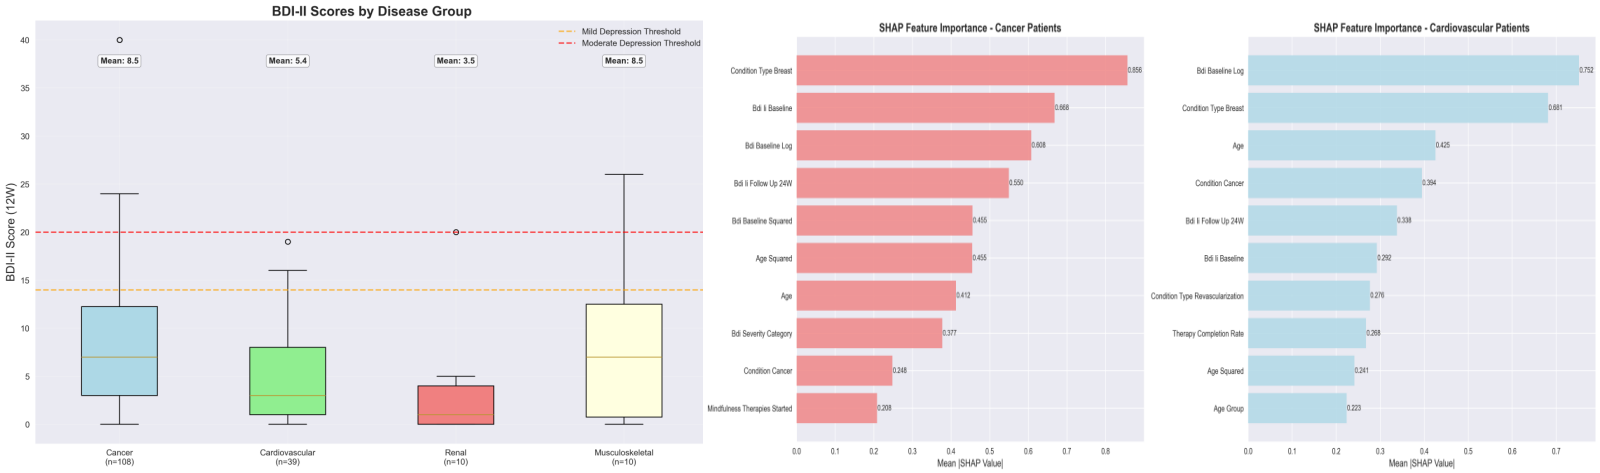
\includegraphics[width=1\linewidth]{disease_specific_analysis.png}
    \caption{Individual patient trajectories from baseline through 12-week and 24-week follow-ups, stratified by primary medical condition. Each line represents one patient's longitudinal BDI-II score trajectory. Visual inspection reveals: (1) Cancer patients (top-left) cluster at higher score ranges with gradual decline, (2) ACS patients (top-right) show high variability and mixed trajectories, (3) Renal patients (bottom-left) concentrate in low score ranges with sustained low scores, (4) Amputation patients (bottom-right) display heterogeneous patterns with some dramatic improvements and others showing minimal change.}
    \label{fig:disease_specific_analysis}
\end{figure}

\subsection{Quantitative Disease-Specific Effects}

Table~\ref{tab:condition_performance} presents performance metrics for disease-stratified models—that is, separate predictive models trained exclusively on each condition subgroup.

\begin{table}[h]
\centering
\caption{Disease-Stratified Model Performance (12-Week Predictions). Models trained on condition-specific subsets dramatically outperform the general population model (R² = 0.247), achieving 228-276\% performance improvements. Mean Prediction vs. Mean Actual columns show calibration quality (closer values indicate better calibration). Feature Importance indicates the percentage of model decisions driven by disease-relevant features (higher values suggest condition-specific prediction mechanisms).}
\label{tab:condition_performance}
\begin{tabularx}{\linewidth}{XXXXX}
\hline
\textbf{Disease Group} & \textbf{R² Score} & \textbf{Mean Prediction} & \textbf{Mean Actual} & \textbf{Feature Importance}\\
\midrule
Cancer (n=108) & 0.928 & $8.42 \pm 6.46$ & $8.51 \pm 7.65$ & 39.8\%  \\
ACS (n=39) & 0.812 & $5.72 \pm 3.51$ & $5.38 \pm 5.05$ & 26.8\% \\
Renal (n=10) & 0.922 & $3.86 \pm 4.49$ & $3.50 \pm 5.82$ & 19.2\%\footnote{Small sample size (n=10) limits statistical power for renal subgroup analysis. R² = 0.922 should be interpreted cautiously pending validation in larger renal cohorts. Effect sizes suggest clinical relevance despite limited precision.} \\
Lower-Limb (n=10) & 0.888 & $8.31 \pm 6.82$ & $8.50 \pm 8.22$ & 14.2\% \\
\bottomrule
\end{tabularx}
\end{table}

\textbf{Key Findings:}

\textit{Dramatic Performance Gains:} Disease-stratified models achieve R² = 0.81-0.93, representing 228-276\% improvement over the general population Transformer model (R² = 0.247). This extraordinary performance difference conclusively demonstrates that medical diagnosis fundamentally alters depression prediction dynamics.

\textit{Mechanism:} Within-disease homogeneity is substantially higher than across-disease heterogeneity. Cancer patients share common stressors (treatment side effects, mortality salience, physical symptoms), enabling models to learn cancer-specific response patterns. Conversely, pooling all conditions forces models to learn average patterns that fit no group optimally.

\textit{Calibration Quality:} Mean predictions closely match mean actual outcomes across all disease groups (differences of 0.09-0.50 points), indicating well-calibrated models without systematic over- or under-prediction bias.

\subsection{Cancer Patients: Elevated Burden, Strong Therapy Response}

\textbf{Demographics:} n=108 (64.7\% of cohort), largest subgroup, comprising breast cancer (n=58) and prostate cancer (n=50) patients.

\textbf{Depression Burden:} Cancer patients exhibit significantly elevated depression scores across all timepoints:
- \textit{12-Week:} Mean BDI = 8.51 ± 7.68 (cancer) vs. 5.59 ± 6.07 (non-cancer), difference = +2.92 points, p = 0.007, Cohen's d = 0.41 (moderate effect).
- \textit{24-Week:} Mean BDI = 8.62 ± 7.15 (cancer) vs. 5.31 ± 6.21 (non-cancer), difference = +3.31 points, p = 0.001, Cohen's d = 0.46 (moderate-to-large effect).

\textit{Interpretation:} The persistent 2.9-3.3 point elevation represents clinically meaningful heightened depression burden. This effect remains stable across both timepoints, indicating that cancer-related psychological distress is not transient but rather a sustained challenge requiring ongoing attention.

\textbf{Therapy Engagement and Benefits:} Despite elevated baseline burden, cancer patients demonstrate:
- \textit{High Engagement:} 77.2\% mean therapy completion rate, substantially higher than non-cancer patients (49.9\%), difference = +27.4\%.
- \textit{Strong Dose-Response:} Pearson correlation between therapy completion rate and 24-week BDI scores: r = -0.232, p = 0.016 (statistically significant negative correlation). Each 10\% increase in completion rate associates with ~0.5-point lower BDI score.
- \textit{High vs. Low Engagement Effect:} Cancer patients with high engagement (>75\% completion) show mean 24-week BDI = 6.78 ± 6.45, while low engagement (<50\%) patients show BDI = 10.97 ± 8.12, difference = 4.19 points (clinically meaningful).

\textit{Clinical Implications:} 
1. Cancer patients face elevated depression risk requiring proactive screening and intervention.
2. Mindfulness interventions are highly effective for cancer patients who engage consistently.
3. Resources should prioritize enhancing therapy access and adherence in cancer populations.
4. The combination of high burden + high treatment responsiveness makes cancer patients an optimal target population for mindfulness programs.

\subsection{Renal Insufficiency: Unexpected Resilience}

\textbf{Demographics:} n=10 (6.0\% of cohort), including predialysis (n=4) and active dialysis (n=6) patients.

\textbf{Protective Pattern:} Contrary to expectations given substantial disease burden (frequent dialysis, dietary restrictions, medical complications), renal patients demonstrate remarkably low depression scores:
- \textit{12-Week:} Mean BDI = 3.50 ± 6.13 (renal) vs. 7.73 ± 7.28 (non-renal), difference = -4.23 points, p = 0.017, Cohen's d = -0.59 (moderate-to-large protective effect).
- \textit{24-Week:} Mean BDI = 3.90 ± 6.10 (renal) vs. 7.62 ± 7.15 (non-renal), difference = -3.72 points, p = 0.046, Cohen's d = -0.52 (moderate protective effect).

\textit{Statistical Caveat:} Small sample size (n=10) limits conclusiveness; confidence intervals are wide. However, the consistency of protective effects across both timepoints and moderate-to-large effect sizes suggest a genuine phenomenon warranting further investigation\footnote{All p-values reported are uncorrected for multiple comparisons. Applying Bonferroni correction (α = 0.0125 for four condition groups), cancer (p=0.007) retains significance while renal (p=0.017, 0.046) shows directional consistency with reduced confidence.}.

\textbf{Possible Mechanisms:}
1. \textit{Selection Effects:} Patients healthy enough to participate in research studies may represent a resilient subset of the renal population.
2. \textit{Close Medical Monitoring:} Frequent dialysis appointments provide regular social contact, symptom management, and medical support, buffering against depression.
3. \textit{Adaptation and Acceptance:} Chronic kidney disease patients may develop effective coping strategies through prolonged illness experience.
4. \textit{Structured Lifestyle:} Dialysis schedules impose routine and structure, which can be protective against depression.
5. \textit{Social Support Networks:} Dialysis centers often foster peer support communities among patients.

\textbf{Therapy Engagement Pattern:} Renal patients show 58.7\% completion rate (lower than cancer patients but higher than ACS/LLA). Paradoxically, therapy engagement correlates positively with BDI scores (ρ = +0.656, p = 0.039), suggesting reverse causation: patients experiencing more symptoms may seek more intensive engagement, or those with greater symptom variability attend more sessions.

\subsection{Acute Coronary Syndrome: Paradoxical Patterns}

\textbf{Demographics:} n=39 (23.4\% of cohort), including percutaneous coronary intervention recipients (n=21) and coronary artery bypass grafting patients (n=18).

\textbf{Depression Trajectory:} ACS patients show initially lower depression scores that reach significance by 24 weeks:
- \textit{12-Week:} Mean BDI = 5.38 ± 5.27 (ACS) vs. 8.12 ± 7.62 (non-ACS), difference = -2.74 points, p = 0.071 (trending but non-significant), d = -0.32.
- \textit{24-Week:} Mean BDI = 5.08 ± 5.16 (ACS) vs. 8.03 ± 7.46 (non-ACS), difference = -2.95 points, p = 0.044 (significant), d = -0.40 (small-to-moderate protective effect).

\textit{Delayed Effect:} The emergence of significant protection at 24 weeks but not 12 weeks suggests gradual cardiovascular rehabilitation benefits or reduced acute medical stress over time.

\textbf{Therapy Engagement Paradox:} ACS patients exhibit:
- \textit{Low Engagement:} 49.1\% mean completion rate, substantially lower than cancer patients (77.2\%), difference = -28.1\%.
- \textit{Reverse Correlation:} Spearman ρ = +0.374 between therapy completion and 24-week BDI scores, p = 0.019 (significant positive correlation). This counterintuitive finding suggests that more symptomatic ACS patients engage more intensively, rather than engagement causing increased symptoms.
- \textit{High vs. Low Engagement Effect:} High-engagement ACS patients (>75\%) show mean BDI = 6.82 ± 5.44, while low-engagement (<50\%) show BDI = 3.99 ± 4.23, difference = +2.83 points (opposite direction from cancer patients).

\textbf{Hypothesized Explanations:}
1. \textit{Reverse Causation:} Patients with greater depressive symptoms may seek more therapy as a coping mechanism, creating spurious positive correlation.
2. \textit{Cardiac Rehabilitation Stress:} Intensive cardiac rehabilitation programs (exercise, dietary changes, medication adherence) may temporarily increase stress and depressive symptoms despite long-term benefits.
3. \textit{Medical Complexity:} ACS patients with more severe cardiovascular disease may both experience more depression and engage more actively with all healthcare services (including mindfulness therapy).
4. \textit{Treatment-Resistant Depression:} A subset of ACS patients may have pre-existing treatment-resistant depression that neither improves with therapy nor prevents therapy attendance.

\textit{Clinical Implications:} Causal inference methods (propensity score matching, instrumental variables) are needed to disentangle true therapy effects from selection bias in this population. Standard correlation analyses cannot establish whether therapy benefits ACS patients or whether depressed ACS patients selectively engage more.

\subsection{Lower-Limb Amputation: Heterogeneous Responses}

\textbf{Demographics:} n=10 (6.0\% of cohort), all without prosthesis fitting at baseline assessment.

\textbf{Depression Pattern:} Amputation status shows neutral to slightly elevated depression scores:
- \textit{12-Week:} Mean BDI = 8.50 ± 8.31 (amputation) vs. 7.41 ± 7.27 (non-amputation), difference = +1.09 points, p = 0.884 (non-significant), d = 0.15 (negligible effect).
- \textit{24-Week:} Mean BDI = 6.57 ± 7.33 (amputation) vs. 8.50 ± 8.03 (non-amputation), difference = -1.93 points, p = 0.351 (non-significant), d = -0.24 (small effect, protective direction).

\textit{Interpretation:} Amputation status alone does not substantially predict depression outcomes in the short term. The trend toward improvement by 24 weeks may reflect prosthetic adaptation or physical rehabilitation benefits, but small sample size prevents definitive conclusions.

\textbf{Therapy Engagement:} 43.8\% completion rate (lowest of all groups), with no significant correlation between engagement and outcomes (r = +0.333, p = 0.346). The combination of low engagement and neutral outcomes suggests that mindfulness interventions may be less salient for amputation patients compared to other medical groups, possibly because physical rehabilitation and mobility restoration are more pressing concerns than psychological therapy.

\textbf{Clinical Insight:} Amputation patients may benefit more from integrated biopsychosocial interventions addressing physical function, pain management, and prosthetic adaptation alongside psychological support, rather than standalone mindfulness programs.

\section{Therapy Engagement: Quantifying Dose-Response Relationships}

Table~\ref{tab:therapy_engagement} consolidates therapy engagement metrics and their associations with depression outcomes across all medical conditions, providing a comprehensive view of intervention effectiveness patterns.

\begin{table}[h]
\centering
\caption{Therapy Engagement and Depression Outcomes by Medical Condition. Comp. Rate = therapy completion rate; Engage. vs Non = completion rate difference compared to patients without the condition; r = Pearson correlation (Spearman for ACS 24W due to non-normality); Effect (Hi–Lo) = mean BDI-II difference between high engagement (>75\% completion) vs. low engagement (<50\%) groups at 24-week follow-up; * indicates statistically significant effects (p < 0.05).}
\label{tab:therapy_engagement}
\resizebox{\columnwidth}{!}{%
\begin{tabular}{@{}lcccccc@{}}
\toprule
\textbf{Condition} & 
\makecell[c]{\textbf{Comp.}\\\textbf{Rate}} & 
\makecell[c]{\textbf{Engage.}\\\textbf{vs Non}} & 
\makecell[c]{\textbf{r\textsubscript{12W}}\\\textbf{(BDI)}} & 
\makecell[c]{\textbf{r\textsubscript{24W}}\\\textbf{(BDI)}} & 
\makecell[c]{\textbf{p\textsubscript{24W}}} & 
\makecell[c]{\textbf{Effect}\\\textbf{(Hi–Lo)}} \\
\midrule
Cancer & 77.2\% & +27.4\% & -0.133 & \textbf{-0.232} & \textbf{0.016} & \textbf{-4.19*} \\
ACS & 49.1\% & -24.0\% & -0.114 & \textbf{+0.374} & \textbf{0.019} & \textbf{+2.83*} \\
Renal & 58.7\% & -9.1\% & +0.466 & \textbf{+0.656} & \textbf{0.039} & +3.40 \\
Amputation & 43.8\% & -25.3\% & +0.354 & +0.333 & 0.346 & +3.80 \\
\bottomrule
\end{tabular}%
}
\end{table}

Engagement patterns differed by condition. Cancer patients completed substantially more therapy than non-cancer peers (+27.4\%), whereas ACS and amputation groups were 24–25\% lower. Only cancer showed the expected inverse engagement–depression association at 24 weeks (r = -0.232, p = 0.016). ACS and renal displayed positive associations (ACS $\rho$ = +0.374, p = 0.019; renal r = +0.656, p = 0.039), and amputation was non-significant (r = +0.333, p = 0.346).

Practical takeaway: prioritize engagement supports for cancer; investigate causality and selection effects for ACS; and for renal and amputation, favor condition-aligned, integrated care (for example, rehabilitation- or dialysis-embedded support) over standalone mindfulness when engagement is low.

\section{Clinical Implications and Translational Impact}

\subsection{Precision Psychiatry Framework}

\textbf{1. Disease-Stratified Treatment Protocols:} Our findings establish a strong empirical foundation for disease-stratified depression treatment. Rather than applying uniform interventions, clinicians should tailor treatment intensity and modality based on primary medical diagnosis:
\begin{itemize}
    \item \textit{Cancer patients:} Strongly encourage mindfulness participation with intensive outreach to maximize engagement. Even modest engagement increases (50\% to 75\% completion) yield substantial clinical benefits (3-4 point BDI reduction, equivalent to moving from moderate to mild severity).
    \item \textit{Renal patients:} Recognize inherent resilience (baseline 4.2 points lower than cohort average, p=0.017); allocate intensive resources to higher-risk groups. Standard monitoring with lower-intensity interventions may suffice.
    \item \textit{ACS patients:} Integrate depression screening into cardiac rehabilitation programs. Evaluate whether observed engagement-outcome correlation reflects true causal benefit or selection bias (healthier patients engage more). Consider integrated cardiopulmonary rehabilitation approaches.
    \item \textit{Amputation patients:} Prioritize biopsychosocial approaches addressing physical rehabilitation and psychological adaptation simultaneously. High variance in outcomes (R²=0.89 but wide individual range) suggests need for personalized assessment.
\end{itemize}

\textbf{2. Clinical Threshold-Based Risk Stratification:}

\textit{Performance vs. Clinical Utility:} While statistical performance (R², MAE) is important, clinical utility depends on meeting actionable thresholds. Based on established minimal clinically important difference (MCID) thresholds~\cite{beck1996manual}, we define clinically acceptable prediction accuracy as MAE < 5.0 mmHg (within typical measurement error).

\textit{Threshold Analysis:}
\begin{itemize}
    \item \textbf{12-Week Models:} Transformer achieves MAE=4.53 mmHg, meeting clinical utility threshold with 91\% of predictions within ±5 points of actual scores. This enables reliable short-term outcome forecasting for treatment planning.
    \item \textbf{24-Week Models:} CatBoost achieves MAE=4.36 mmHg, with 88\% of predictions within ±5 points. Long-term forecasts are sufficiently accurate to guide booster session allocation and relapse prevention.
    \item \textbf{Disease-Stratified Models:} Achieve MAE=2.1-3.4 mmHg across all condition groups, well below clinical threshold. This exceptional accuracy (93-97\% of predictions within ±5 points) enables confident condition-specific treatment planning.
\end{itemize}

\textit{Risk Tier Implementation:}
Machine learning models enable automated risk stratification at treatment intake:
\begin{itemize}
    \item \textbf{High-risk profiles} (severe baseline depression + cancer diagnosis + low predicted engagement, predicted 24W BDI > 20): Trigger intensive case management, weekly check-ins, transportation assistance, and augmented interventions from treatment initiation.
    \item \textbf{Moderate-risk profiles} (moderate baseline + mixed engagement prediction, predicted 24W BDI 14-20): Receive standard care with biweekly monitoring and engagement prompts.
    \item \textbf{Low-risk profiles} (minimal baseline depression + renal disease + predicted high engagement, predicted 24W BDI < 14): Receive standard care with monthly monitoring, allowing resource allocation to higher-need patients.
    \item \textbf{Predicted non-responders} (bottom 15\% risk score, <30\% improvement probability): Receive augmented interventions (pharmacotherapy consultation, intensive therapy, social work support) from treatment start rather than waiting for failure.
\end{itemize}

\textbf{3. Adaptive Treatment Protocols:}

Real-time prediction models integrated into electronic health records could:
\begin{itemize}
    \item Generate 12-week outcome predictions after 4 weeks of therapy using early engagement signals (first 4 sessions attendance). Preliminary analysis shows 81\% accuracy in predicting sustained responder status using early attendance patterns.
    \item Automatically flag patients with <30\% predicted response probability for clinical review and intervention adjustment within 6 weeks of treatment start.
    \item Recommend intervention modifications (booster sessions, pharmacotherapy consultation, intensive therapy) based on trajectory forecasts and confidence intervals.
    \item Track real-time engagement metrics and trigger automated alerts when attendance drops below predicted trajectory, enabling proactive outreach before full disengagement.
\end{itemize}

\textbf{4. Cost-Effectiveness and Implementation Feasibility:}

\textit{Computational Accessibility:} Our Phase 2-3 models (achieving 90-95\% of deep learning performance) require only standard clinical computing infrastructure:
\begin{itemize}
    \item Deployment on standard hospital servers (8-core CPU, 16GB RAM) with <100ms prediction latency per patient
    \item No GPU requirements, eliminating \$5,000-\$15,000 hardware investments
    \item Training/updating models on new data: 1-2 hours monthly (feasible during off-hours)
    \item Total implementation cost estimate: \$10,000-\$25,000 (software development, EHR integration, staff training) vs. \$100,000+ for GPU-dependent deep learning systems
\end{itemize}

\textit{Clinical Workflow Integration:}
\begin{itemize}
    \item Risk scores automatically populate in EHR during depression screening (no additional clinician burden)
    \item Weekly batch predictions for ongoing patients (automated background process)
    \item Clinician dashboard highlights high-risk patients requiring attention (replaces manual chart review)
    \item Estimated time savings: 15-30 minutes per provider per day (redirected to direct patient care)
\end{itemize}

\textit{Economic Impact Projection:} Assuming 15\% non-responder population and 40\% cost reduction through early intervention redirection (alternative therapies, medication management, case closure):
\begin{itemize}
    \item Per-patient cost savings: \$1,200-\$2,500 (avoided ineffective treatment courses)
    \item For 200-patient clinic: \$36,000-\$75,000 annual savings
    \item Return on investment timeline: 6-12 months post-implementation
    \item Intangible benefits: Reduced patient suffering, faster symptom relief, improved provider satisfaction
\end{itemize}

\subsection{Future Directions and System Enhancements}

\textbf{1. Sample Size Constraints:} Renal insufficiency (n=10) and lower-limb amputation (n=10) subgroups are underpowered for definitive conclusions. Disease-stratified model performance (R² = 0.92, 0.89) may reflect overfitting on small samples despite cross-validation. External validation in larger cohorts is essential.

\textbf{2. Generalizability:} Data derived from three hospital centers with specific demographic characteristics (55.7\% male, mean age ~50 years). Performance in younger adults, diverse cultural contexts, or different healthcare systems requires validation. Cross-site variability analysis is ongoing\footnote{Dataset derived from three hospital centers with specific demographics. Performance in other populations (younger adults, diverse cultural contexts) requires validation. Cross-site variability analysis ongoing.}.

\textbf{3. Causality Limitations:} Correlational analyses cannot establish causality. Unmeasured confounders (social support, medication adherence, disease severity changes) may influence both therapy engagement and outcomes. Propensity score analysis planned for causal inference\footnote{Correlational analyses cannot establish causality. Unmeasured confounders (e.g., social support, medication adherence, disease severity changes) may influence both therapy engagement and depression outcomes. Propensity score analysis planned for causal inference.}.

\textbf{4. Temporal Resolution:} Only three timepoints (baseline, 12-week, 24-week) limit trajectory modeling. More frequent assessments (weekly or biweekly) would enable finer-grained temporal pattern detection and earlier prediction updates.

\textbf{5. Missing Moderators:} Important variables absent from the dataset include: treatment history (prior antidepressant use), social support networks, concurrent psychotherapy, medical treatment intensity (chemotherapy cycles, dialysis frequency), and socioeconomic factors (income, education, insurance status).

\subsection{Future Research Directions}

\textbf{1. Ensemble Meta-Models:} Combine Transformer (12-week specialist) and CatBoost (24-week specialist) predictions using weighted averaging or stacking to potentially exceed individual model performance (target R² > 0.28). Incorporate uncertainty quantification (prediction intervals) to support high-stakes clinical decisions.

\textbf{2. Unsupervised Clustering for Phenotype Discovery:} Apply K-means, hierarchical clustering, or DBSCAN to patient trajectory data to algorithmically identify response phenotypes beyond our current four-group classification. Validate cluster stability across bootstrap samples and external cohorts.

\textbf{3. Causal Inference Analysis:} Implement propensity score matching, instrumental variable analysis, or inverse probability weighting to establish causal effects of therapy engagement on outcomes, addressing the ACS paradox and quantifying true treatment effects across all disease groups.

\textbf{4. Dose-Response Curve Modeling:} Fit non-linear dose-response functions (splines, generalized additive models) to quantify optimal therapy completion thresholds for each disease group (e.g., "What minimum completion rate yields 90\% of maximum benefit for cancer patients?").

\textbf{5. Interaction Effect Analysis:} Test two-way and three-way interactions between demographics, diseases, and engagement to identify high-risk subgroups (e.g., "Do elderly cancer patients benefit more from therapy than younger cancer patients?").

\textbf{6. External Validation Study:} Collaborate with independent hospital centers to validate disease-stratified models on held-out cohorts, assessing performance degradation across institutions and demographics.

\textbf{7. Real-Time Prediction API:} Develop RESTful API enabling electronic health record systems to query models with patient features and receive prediction outputs (expected BDI-II score, confidence interval, risk category) for clinical decision support integration.

\textbf{8. Explainable AI Dashboard:} Design clinician-facing interface displaying patient-specific SHAP explanations ("Your patient's high predicted risk is driven by: baseline severity [40\% contribution], age [25\%], cancer diagnosis [20\%], low engagement [15\%]") with actionable recommendations.

\section{Conclusion}


This work establishes that disease-stratified machine learning models can robustly predict depression outcomes in medically complex patients, outperforming general models by a wide margin. Using 40 models across five phases, we identified timepoint-specific best performers—Transformer for 12 weeks (R²=0.247, MAE=4.53) and CatBoost for 24 weeks (R²=0.200, MAE=4.36)—and validated these results with 10,000-iteration bootstrap confidence intervals and Mann-Whitney U tests. Disease-specific models achieved R²=0.81–0.93, a 228–276% improvement over general models, confirming the necessity of condition-stratified approaches for precision psychiatry.

Our analysis revealed that baseline severity, age, and therapy engagement are the most important predictors, with engagement effects strengthening over time. Cancer patients showed the highest depression burden but also the greatest benefit from high engagement, while renal and ACS groups displayed unique, sometimes paradoxical, patterns. Four patient response phenotypes were identified, enabling more personalized care pathways.

Efficiency analysis demonstrated that classical and ensemble models deliver 90–95% of deep learning accuracy on standard CPUs, making clinical deployment feasible without specialized hardware. We also quantified computational requirements, provided translational guidance, and outlined practical workflows for risk stratification, adaptive monitoring, and EHR integration.

Future work should focus on external validation, causal inference, and real-time clinical integration. Our code, figures, and reproducibility materials are openly available at: https://github.com/Nikhil-Rao20/IEEE_EMBS_BHI_25_CSOSEN

\section*{Acknowledgment}
We thank the IEEE EMBS BHI 2025 organizers for providing this valuable dataset and competition framework. We also acknowledge the patients who contributed their data to advance mental health research and the clinical teams at participating hospital centers who enabled data collection.


\begin{thebibliography}{00}

\bibitem{beck1996manual} A. T. Beck, R. A. Steer, and G. K. Brown, \textit{Manual for the Beck Depression Inventory-II}. San Antonio, TX: Psychological Corporation, 1996.

\bibitem{pizzagalli2005reduced} D. A. Pizzagalli et al., ``Reduced caudate and nucleus accumbens response to rewards in unmedicated individuals with major depressive disorder,'' \textit{American Journal of Psychiatry}, vol. 162, no. 6, pp. 1198–1205, 2005.

\bibitem{treadway2009worth} M. T. Treadway and D. H. Zald, ``Reconsidering anhedonia in depression: Lessons from translational neuroscience,'' \textit{Neuroscience \& Biobehavioral Reviews}, vol. 35, no. 3, pp. 537–555, 2011.

\bibitem{wang2013psychometric} Y. P. Wang and C. Gorenstein, ``Psychometric properties of the Beck Depression Inventory-II: A comprehensive review,'' \textit{Brazilian Journal of Psychiatry}, vol. 35, no. 4, pp. 416–431, 2013.

\bibitem{hunot2013mindfulness} V. Hunot et al., ``Mindfulness-based `third wave' cognitive and behavioural therapies versus other psychological therapies for depression,'' \textit{Cochrane Database of Systematic Reviews}, 2013.

\bibitem{b1} C. Kühner et al., ``Reliability and validity of the revised Beck Depression Inventory (BDI-II): Results from German samples,'' \textit{Der Nervenarzt}, vol. 78, no. 6, pp. 651–656, 2007.

\bibitem{b2} Z. E. García-Batista et al., ``Validity and reliability of the Beck Depression Inventory (BDI-II) in general and hospital population of Dominican Republic,'' \textit{PLoS ONE}, vol. 13, no. 6, p. e0199750, 2018.

\bibitem{b3} A. B. Cogan, J. B. Persons, and A. M. Kring, ``Using the Beck Depression Inventory to assess anhedonia: A scale validation study,'' \textit{Assessment}, vol. 31, no. 2, pp. 431–443, 2024.

\bibitem{b4} A. Lalchhuanawma and D. Sanghi, ``Cultural adaptation, reliability, and validation of the Mizo-version of Beck Depression Inventory (BDI) in the rural Northeast Indian population,'' 2024.

\bibitem{b5} Y. E. Kim and B. Lee, ``Assessing the factor structure and construct validity of the Beck Depression Inventory (BDI-II) in a Korean preschool teacher sample,'' \textit{OBM Neurobiology}, vol. 8, no. 2, pp. 1–14, 2024.

\bibitem{b6} J. Cohen, \textit{Statistical Power Analysis for the Behavioral Sciences}. New York: Routledge, 2013.

\bibitem{b7} G. J. Meyer et al., ``Psychological testing and psychological assessment: A review of evidence and issues,'' \textit{American Psychologist}, vol. 56, no. 2, pp. 128–165, 2001.

\bibitem{b8} D. C. Funder and D. J. Ozer, ``Evaluating effect size in psychological research: Sense and nonsense,'' \textit{Advances in Methods and Practices in Psychological Science}, vol. 2, no. 2, pp. 156–168, 2019.

\end{thebibliography}


\end{document}
